\documentclass[12pt,a4paper,twoside]{report}

\usepackage[utf8x]{inputenc}
\usepackage[english,hebrew]{babel}

\usepackage{graphicx}
\usepackage{verbatim}
\usepackage{url}
\usepackage{bm}
\usepackage{float}
\usepackage{eqnarray}

\usepackage{tikz}
\usepackage{tkz-euclide}
\usepackage{pgfplots}
\usetikzlibrary{positioning,through,calc,intersections,arrows.meta,external}
%\tikzexternalize[prefix=tikz/]
\tikzset{>=stealth} % Use stealth arrows
\usetkzobj{all}

\textwidth=155mm
\textheight=235mm
\topmargin=0pt
\headheight=0pt
\oddsidemargin=-5mm
\evensidemargin=5mm
\headsep=0pt
\parindent=0pt
\renewcommand{\baselinestretch}{1.1}
\setlength{\parskip}{0.3\baselineskip plus 1pt minus 1pt}

\graphicspath{{images/}}

\newcommand*{\p}[1]{\textsf{\small #1}}
\newcommand*{\bover}[1]{\bm{\overline{#1}}}
\newcommand*{\erh}[1]{\setlength{\extrarowheight}{#1}}
\newcommand*{\np}{\selectlanguage{english}\newpage\selectlanguage{hebrew}}
\newcommand*{\disfrac}[2]{\displaystyle\frac{#1}{#2}}
\newcommand*{\asm}{אסימפטוטה}
\newcommand*{\asms}{אסימפטוטות}


%  Less space above chapter title
\makeatletter
\def\@makechapterhead#1{%
  {\parindent \z@ \raggedright \normalfont
    \ifnum \c@secnumdepth >\m@ne
        \centering\huge\bfseries \@chapapp\space \thechapter
        \hspace{.3em}
    \fi
    \Huge \bfseries #1\par\nobreak
    \vskip 20\p@
  }}
\makeatother

\selectlanguage{hebrew}


\includeonly{rational}

\begin{document}

% !TeX root = chapter-6-7-8.tex

\selectlanguage{hebrew}

\thispagestyle{empty}

\begin{center}
\textbf{\LARGE בחינות בגרות במתמטיקה: החוויה}

\bigskip
\bigskip

\textbf{\LARGE חשבון דיפרנציאלי ואינטגרלי}

\bigskip
\bigskip
\bigskip
\bigskip

\textbf{\Large מוטי בן-ארי}

\bigskip
\bigskip

\url{http://www.weizmann.ac.il/sci-tea/benari/}
\end{center}

% !TeX root = construct.tex

\begin{center}
\begin{bfseries}
\bigskip
\bigskip

Version 2.1

\bigskip

\today

\end{bfseries}
\end{center}


\vfill

\selectlanguage{english}

\begin{footnotesize}
\begin{center}
\copyright{}\ 2017--19 by Moti Ben-Ari.
\end{center}

This work is licensed under the Creative Commons Attribution-ShareAlike 3.0 Unported License. To view a copy of this license, visit \url{http://creativecommons.org/licenses/by-sa/3.0/} or send a letter to Creative Commons, 444 Castro Street, Suite 900, Mountain View, California, 94041, USA.
\end{footnotesize}

\bigskip

\begin{center}

\includegraphics[width=.15\textwidth]{../../by-sa.png}
\end{center}

\np
\thispagestyle{empty}
\mbox{}
\np
\thispagestyle{empty}

\tableofcontents
\np

\section*{הקדמה}
\addcontentsline{cot}{section}{הקדמה}

בנוסחאון נתון:
\[
\textrm{(\R{ממשי} t)} \quad\quad (x^t)' = tx^{t-1}\,,
\]
אולם משתמשים בנוסחה רק עבור 
$t$
שלם וחיובי. אני מעדיף להשתמש בנוסחה עבור כל
$t$
כי קל לזכור את הנוסחה והחישובים פשוטים. למשל, הנוסחה הנתונה 
\[
(\sqrt{x})' = \disfrac{1}{2\sqrt{x}}
\]
מיותרת כי:
\[
(\sqrt{x})' = (x^\frac{1}{2})'= \frac{1}{2}(x^{-\frac{1}{2}}) = \frac{1}{2}\cdot\frac{1}{x^{\frac{1}{2}}}=\disfrac{1}{2\sqrt{x}}\,.
\]
החיסכון בולט יותר כאשר מנסים לחשב נגזרת רציונלית:
\[
\left(\frac{1}{x^t}\right)'\,.
\]
משתמשים בנוסחה המובכת עבור נגזרת של מנה כאשר
$f(x)=1, g(x)=x^t$.
לדעתי, פשוט יותר לחשב:
\[
\left(\frac{1}{x^t}\right)'=(x^{-t})'=-t(x^{-t-1})=\frac{-t}{x^{t+1}}\,.
\]
כאשר במנה יש קבוע ובמכנה יש פונקציה מורכבת החישוב לא מסובך במיוחד. למשל:
\erh{12pt}
\begin{equationarray*}{rcl}
\left(\frac{14}{x^2-3x+4}\right)'&=&14\left((x^2-3x+4)^{-1}\right)'\\
&=&14\cdot -1\cdot (x^2-3x+4)^{-2}(x^2-3x+4)'\\
&=&-14(x^2-3x+4)^{-2}(2x-3)\\
&=&\frac{-14(2x-3)}{(x^2-3x+4)^{-2}}\,.
\end{equationarray*}


כמובן שאתם חופשיים להשתמש בנוסחאות האחרות.

\selectlanguage{english}

\tikzsetfigurename{rational}
% !TeX root = chapter-6-7-8.tex

\selectlanguage{hebrew}


\begin{comment}

\chapter{חקר פונקציות רציונליות}

%%%%%%%%%%%%%%%%%%%%%%%%%%%%%%%%%%%%%%%%%%%%%%%%%%%%%%%%%%%%%%%%%%%%%%


\section{קיץ תשע"ח מועד ב}

\begin{center}
\selectlanguage{english}
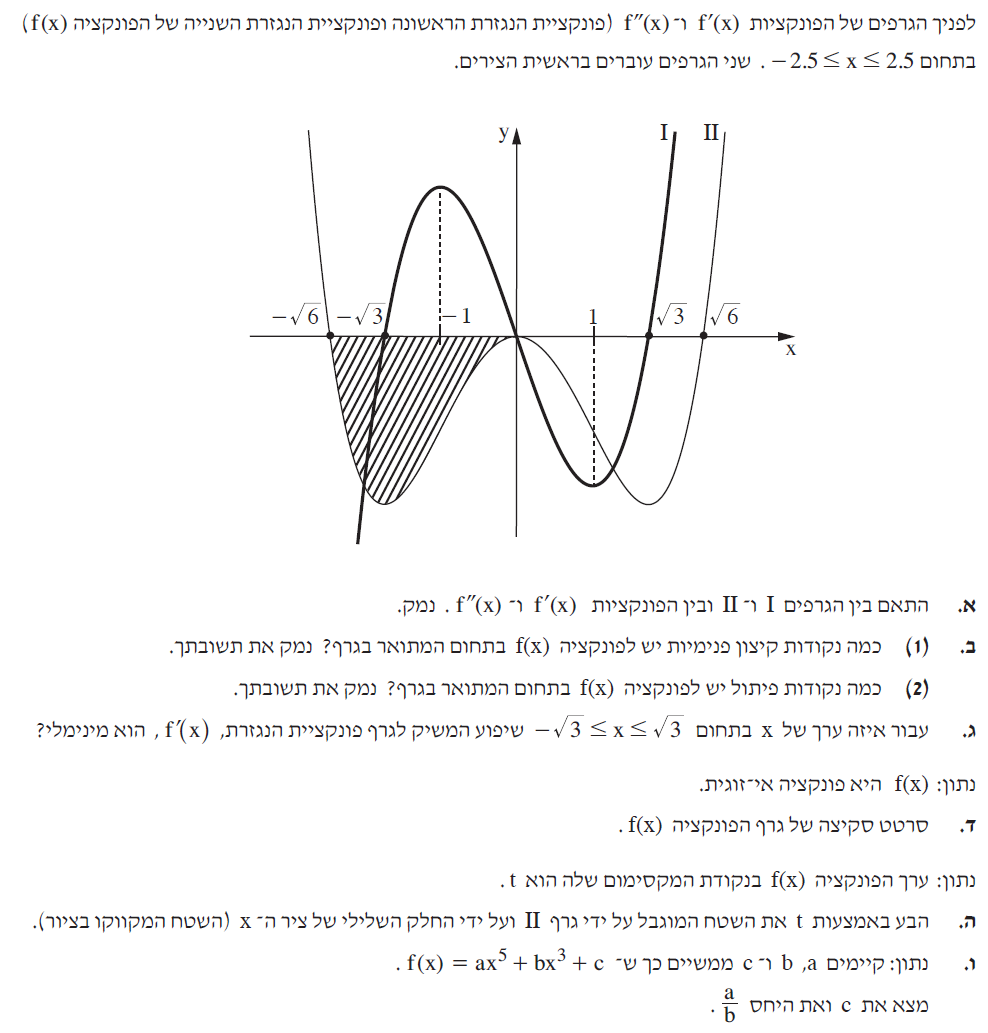
\includegraphics[width=\textwidth]{summer-2018b-6}
\end{center}

\vspace{-4ex}

\textbf{סעיף א}

נקודות הקיצון של
$f'(x)$
יהיו הנקודות בהן 
$f''(x)=0$.
לגרפ
$II$
נקודות קיצון ב-%
$\pm\sqrt{3},0$
ובנקודות הללו הגרף
$I$
חותך את ציר ה-%
$x$.
לכן, 
$II$
הוא הגרף של
$f'(x)$
ו-%
$I$
הוא הגרף של
$f''(x)$.

\textbf{סעיף ב}

$(1)$
הגרף 
$II$
מתאפס ב-%
$\pm\sqrt{6},0$,
אבל ב-%
$0$
הוא לא מחליף סימן ולכן
$0$
הוא לא נקודת קיצון.

$(2)$
הנגזרת השנייה מתאפסת בשלוש נקודות
$\pm\sqrt{6},0$.
בכל שלושת הנקודות הנגזרת הראשונה לא מחליפה סימן, ולכן כולן נקודות פיתול ולא נקודות קיצון.

\textbf{סעיף ג}

הנגזרת השנייה היא שיפוע המשיק לנגזרת הראשונה. בתחום הניתן הערך המינימלי מתקבל ב-%
$1$.

\np

\textbf{סעיף ד}

נתון שהפוקציה אי-זוגית אז 
$f(0)=0$.
\begin{quote}
$a=-a$
אם ורק אם
$a=0$.
אם
$f(x)$
אי-זוגית,
$f(0)=f(-0)=-f(0)=0$.
\end{quote}
בסעיף ב חישבנו שיש שתי נקודות פיתול נוספות
$\pm\sqrt{6}\approx 2.45$,
והגרף נראה כך:
\begin{center}
\selectlanguage{english}
\begin{tikzpicture}[scale=1]
\begin{axis}[
    xlabel = $x$,
    ylabel = {$f(x)$},
    axis lines=center,
    xmin = -2.51,
    xmax = 2.51,
    ymin = -60,
    ymax = 60,
    every axis y label/.style={at={(ticklabel cs:0.7)},rotate=90,anchor=west,},
    every axis x label/.style={at={(ticklabel cs:0.9)},anchor=north,},
]
\addplot [
    domain=-2.5:2.5, 
    samples=50, 
]
{x^5-10*x^3};
\draw[dashed,thick] ({axis cs:2.45,0}|-{rel axis cs:0,0}) -- ({axis cs:2.45,0}|-{axis cs:0,0});
\draw[dashed,thick] ({axis cs:-2.45,0}|-{rel axis cs:0,2}) -- ({axis cs:-2.45,0}|-{axis cs:0,0});
\end{axis}
\end{tikzpicture}
\end{center}

\textbf{סעיף ה}

לפי הנתון שהפונקציה א-זוגית
$f(0)=0$,
לכן יש לנו את גבולות האינטגרל:
\[
\int_{-\sqrt{6}}^0 0-f'(x) dx = - \left.f(x)\right|_{-\sqrt{6}}^{0}=-(-f(-\sqrt{6}))=t\,,
\]
כי נקודת המקסימום של 
$f(x)$
היא הנקודה בה הנגזרת הראשונה עוברת מחיובי לשלילי
$-\sqrt{6}$.

\textbf{סעיף ו}

לפי
$f(0)=0$,
$c=0$.

הנגזרצ הראשונה מתאפסת ב-%
$\pm\sqrt{6}$:
\erh{0pt}
\begin{equationarray*}{rcl}
f'(x) &=& 5ax^4 + 3bx^2\\
&=& 5a(\sqrt{6})^4 + 3b(\sqrt{6})^2= 0\\
5a(\sqrt{6})^2 + 3b&=& 0\\
30a+3b&=&0\\
\frac{a}{b}&=&-\frac{1}{10}\,.
\end{equationarray*}


%%%%%%%%%%%%%%%%%%%%%%%%%%%%%%%%%%%%%%%%%%%%%%%%%%%%%%%%%%%%%%%%%%%%%%


\section{קיץ תשע"ח מועד א}

\begin{center}
\selectlanguage{english}
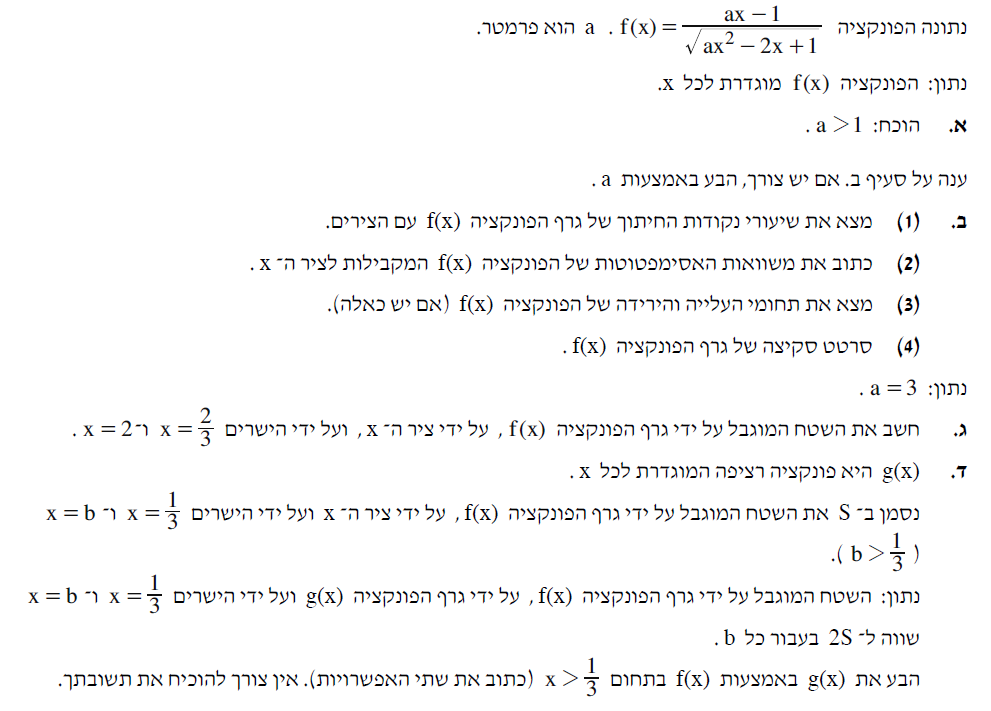
\includegraphics[width=\textwidth]{summer-2018a-6}
\end{center}

\vspace{-4ex}

\textbf{סעיף א}

המכנה לא יכול להיות אפס. לפולינום הריבוע יהיו פתרונות אם
$(-2)^2-4\cdot a \cdot 1 = 4-4a\geq 0$,
ולכן 
$a>1$.
עלינו לוודא שהפולינום לא מקבל ערכים שליליים כדי שהשורש יהיה מוגדר. ללא קשר לערך של 
$a$,
הערך של הפולינום הוא
$1$,
כלומר, יש לו ערך חיובי אחד לפחות. אם אין פתרונות לפולינום, אז אין חיתוכים עם ציר ה-%
$x$
ולא יהיו ערכים שליליים.

\textbf{סעיף ב}

$(1)$
$f(0)=\frac{-1}{\sqrt{1}}$
ונקודת החיתוך עם ציר ה-%
$y$
היא
$(0,-1)$.

$(2)$
המכנה חיובי כך שנקודת החיתוך עם ציר ה-%
$x$
מתקבל מ-%
$ax-1=0$,
והנקודה היא
$(\frac{1}{a},0)$.

$(3)$

\vspace{-3ex}

\erh{12pt}
\begin{equationarray*}{rcl}
f(x)&=&\frac{ax-1}{\sqrt{ax^2-2x+1}}\\
&=&\frac{x(a-\frac{1}{x})}{\sqrt{x^2}\left(\sqrt{a-\frac{2}{x}+\frac{1}{x^2}}\right)}\\
&\mathop{\longrightarrow}\limits_{\pm\infty}&\frac{xa}{\sqrt{x^2}\sqrt{a}}\,.
\end{equationarray*}
ה%
\asms{}
הן
$f(x)\mathop{\longrightarrow}\limits_{+\infty}\sqrt{a}$,
$f(x)\mathop{\longrightarrow}\limits_{-\infty}-\sqrt{a}$.

\np

$(4)$
\erh{16pt}
\begin{equationarray*}{rcl}
f'(x)&=&\frac{a\sqrt{ax^2-2x+1}-\disfrac{(ax-1)(2ax-2)}{2\sqrt{ax^2-2x+1}}}{(\sqrt{ax^2-2x+1})^2}\\
&=&\frac{a(ax^2-2x+1)-(ax-1)(ax-1)}{(\sqrt{ax^2-2x+1})^2\sqrt{ax^2-2x+1}}\,.
\end{equationarray*}
המכנה חיובי ולכן סימן הנגזרת תלוי בסימן המונה:
\[
a^2x^2-2ax+a-a^2x^2+2ax-1=a-1\,.
\]
הוכחנו ש-%
$a>1$
ולכן
$a-1>0$
והפונקציה תמיד עולה.

$(4)$

\vspace{-4ex}

\begin{center}
\selectlanguage{english}
\begin{tikzpicture}[scale=1]
\begin{axis}[
    xlabel = $x$,
    ylabel = {$f(x)$},
    axis lines=center,
    xtick={-4,...,4},
    ytick={-2,...,2},
    xmin = -4,
    xmax = 4,
    ymin = -2,
    ymax = 2,
    yticklabel style={
    anchor=east,
    },
    every axis y label/.style={at={(ticklabel cs:0.7)},rotate=90,anchor=west,},
    every axis x label/.style={at={(ticklabel cs:0.9)},anchor=north,},
]
\addplot [
    domain=-4:4, 
    samples=50, 
]
{(3*x-1)/sqrt(3*x^2-2*x+1)};
\draw[dashed,thick] ({axis cs:-4,-1.732}-|{rel axis cs:0,0}) -- ({axis cs:-4,-1.732}-|{rel axis cs:8,0});
\draw[dashed,thick] ({axis cs:-4,1.732}-|{rel axis cs:0,0}) -- ({axis cs:-4,1.732}-|{rel axis cs:8,0});
\fill (axis cs:0,-1) circle(1.5pt) node[right] {$(0,-1)$};
\fill (axis cs:.333,0) circle(1.5pt) node[above right] {$(1/3,0)$};
\end{axis}
\end{tikzpicture}
\end{center}

\textbf{סעיף ג}

$\frac{1}{3}<\frac{2}{3}$
ולכן גבולות האינטגרל בחלק החיובי של הפונקציה.
\erh{12pt}
\begin{equationarray*}{rcl}
\int_{2/3}^2 \frac{3x-1}{\sqrt{3x^2-2x+1}}&=& \int_{2/3}^2 \frac{2}{2}\left(\sqrt{3x^2-2x+1}\right)'\\
&=&\left. \sqrt{3x^2-2x+1} \right|_{2/3}^2\\
&=&{\sqrt{12-4+1}}-\sqrt{\frac{4}{3}-\frac{4}{3}+1}=3-1=2\,.
\end{equationarray*}

\vspace{-4ex}

\textbf{סעיף ד}

שתי האפשרויות הן ש-%
$f(x)$
מעל 
$g(x)$
וש-%
$g(x)$
מעל
$f(x)$.
\[
\int (g-f) = \int g - \int f = \int g - S = 2S\,,
\]
ולכן
$\int g = 3S$,
$g=3f$.

\[
\int (f-g) = \int f - \int g = S-\int g= 2S\,,
\]
ולכן
$-\int g = S$,
$g=-f$.

%%%%%%%%%%%%%%%%%%%%%%%%%%%%%%%%%%%%%%%%%%%%%%%%%%%%%%%%%%%%%%%%%%%%%%

\section{חורף תשע"ח}

\begin{center}
\selectlanguage{english}
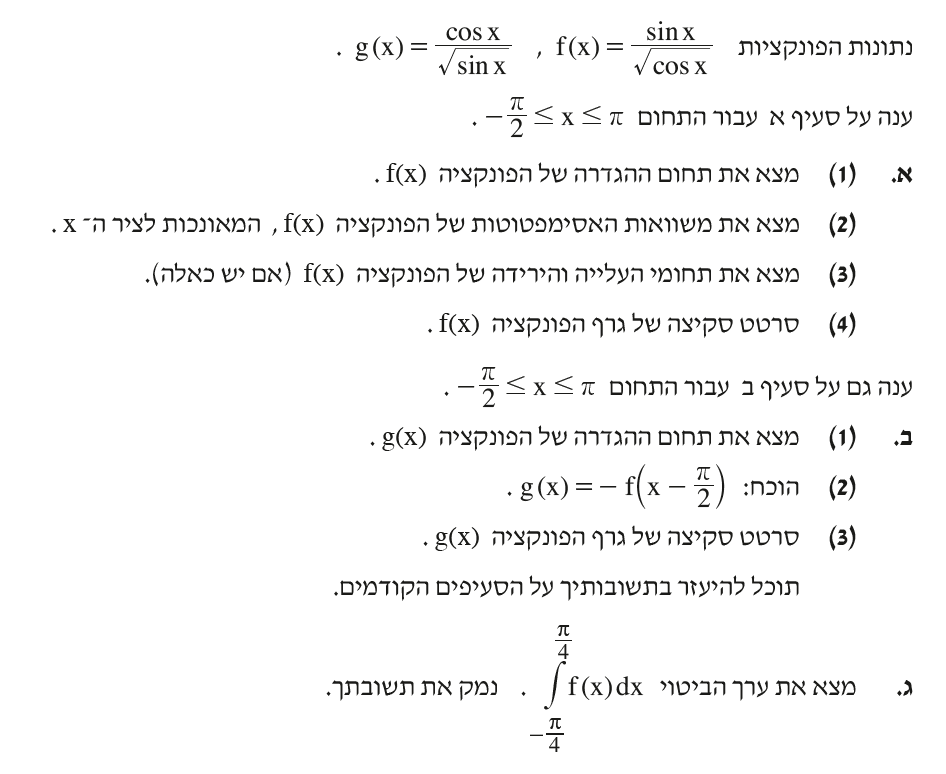
\includegraphics[width=\textwidth]{winter-2018-6}
\end{center}

\vspace{-4ex}

התרשים להלן יאפשר לנו לחשב תכונות של הפונקציות הטריגונומטריותת. הקשת העבה מראה את התחום בשאלה והקווים המקווקווים מראים איך מתקבל
$x-\disfrac{\pi}{2}$
)סעיף ב-%
$2$(.

\vspace{-2ex}

\begin{center}
\selectlanguage{english}
\begin{tikzpicture}[scale=.8]
\coordinate (O) at (0,0);
\coordinate (A) at (0,-2);
\node[draw,circle through=(A)] at (O) {};
\draw (-2,0) -- (2,0);
\draw (0,-2) -- (0,2);
\draw[ultra thick] (A) arc[start angle=-90,end angle=180,radius=2];
\node[right] at (2,0) {$0$};
\fill ($(O)+(-90:2)$) circle(2pt) node[below] {$-\pi/2$};
\fill ($(O)+(90:2)$) circle(2pt) node[above] {$\pi/2$};
\fill ($(O)+(180:2)$) circle(2pt) node[left] {$\pi$};
\draw[thick,dashed] (O) -- (30:2) node[above right] {$\pi/6$};
\draw[thick,dashed] (O) -- (-60:2) node[below right] {$-\pi/3$};
\end{tikzpicture}
\end{center}

\vspace{-2ex}

\textbf{סעיף א}

$(1)$
הפונקציה מוגדרת אם
$\cos x>0$:
אם 
$x$
מימין לציר ה-%
$y$.
תחום ההגדרה הוא
$-\frac{\pi}{2}<x<\frac{\pi}{2}$.

$(2)$
\[
\frac{\sin x}{\sqrt{\cos x}} \mathop{\longrightarrow}\limits_{+\infty} \frac{+1}{0}\mathop{\longrightarrow}\limits_{+\infty} +\infty,\quad\quad \frac{\sin x}{\sqrt{\cos x}} \mathop{\longrightarrow}\limits_{-\infty} \frac{-1}{0}\mathop{\longrightarrow}\limits_{-\infty} -\infty
\]

\np

$(3)$
\erh{12pt}
\begin{equationarray*}{rcl}
f'(x) &=& \frac{\cos x\sqrt{\cos x} - \sin x \cdot\frac{-\sin x}{2\sqrt{\cos x}}}{\cos x}\\
&=& \frac{2\cos^2 x + \sin^ x}{2\cos x\sqrt{\cos x}}\\
&=& \frac{\cos^2 x + 1}{2\cos x\sqrt{\cos x}}\,.
\end{equationarray*}

\vspace{-3ex}

בתחום ההגדרה
$\cos x > 0$
ולכן הנגזרת הראשונה תמיד חיובית והפונקציה עולה בכל התחום. )ברור שאם הנגזרת תמיד חיובית, היא לא מתאפסת בתחום כך שאין נקודות קיצון פנימיות.(

$(4)$
\begin{center}
\selectlanguage{english}
\begin{tikzpicture}[scale=.9]
\begin{axis}[
    axis lines=center,
    xtick={-90,0,90,180},
    xticklabels={$-\disfrac{\pi}{2}$,$0$,$\disfrac{\pi}{2}$,$\pi$},
    xticklabel style={
    anchor=north east,
    },
    ymajorticks=false,
    xmin = -90.1,
    xmax = 180,
    ymin = -2,
    ymax = 2,
]
\addplot [
    domain=-89:79, 
    samples=40, 
]
{(sin(x)/(sqrt(cos(x))};
\draw[dashed,thick] ({axis cs:-90,-2}|-{rel axis cs:0,0}) -- ({axis cs:-90,0}|-{rel axis cs:0,4});
\draw[dashed,thick] ({axis cs:90,-2}|-{rel axis cs:0,0}) -- ({axis cs:90,0}|-{rel axis cs:0,4});
\end{axis}
\end{tikzpicture}
\end{center}

\textbf{סעיף ב}

$(1)$
הפונקציה מוגדרת אם
$\sin x>0$:
אם 
$y$
מעל לציר ה-%
$x$.
תחום ההגדרה הוא
$0<x<\pi$.

$(2)$
חיבור או חיסור של
$\frac{\pi}{2}$
משנה סינוס לקוסינוס ולהיפך. קל להשתכנע כי במשולש ישר זווית, הזוויות החדות הן
$\theta$, $\frac{\pi}{2}-\theta$.
צריך רק לקבוע את הסימנים, ובתרשים הראשון אנו רואים שסימן הקוסינוס נשאר חיובי והסימן של הסינוס משנה סימן:
\[
f\left(\frac{\pi}{2}-x\right)=\frac{-\cos x}{\sqrt{\sin x}}=-g(x)\,.
\]
אפשר גם לחשב לפי הנוסחה לחיסור של סינוס וקוסינוס:
\erh{6pt}
\begin{equationarray*}{rcl}
\sin \left(x-\frac{\pi}{2}\right)&=&\sin x \cos \frac{\pi}{2}-\cos x\sin \frac{\pi}{2}=0\cdot \sin x-1\cdot \cos x=-\cos x\\
\cos \left(x-\frac{\pi}{2}\right)&=&\cos x \cos \frac{\pi}{2}+\sin x\sin \frac{\pi}{2}=0\cdot \cos x+1\cdot \sin x=\sin x\,.
\end{equationarray*}

\np

$(3)$
הגרף של 
$g(x)$
מתקבל מהזזה ימינה של
$\frac{\pi}{2}$
והפיכת הסימן. למשל
\[
g\left(\frac{\pi}{2}\right)=-f\left(\frac{\pi}{2}-\frac{\pi}{2}\right)=-f(0)\,.
\]
\begin{center}
\selectlanguage{english}
\begin{tikzpicture}[scale=.9]
\begin{axis}[
    axis lines=center,
    xtick={-90,0,90,180},
    xticklabels={$-\disfrac{\pi}{2}$,$0$,$\disfrac{\pi}{2}$,$\pi$},
    xticklabel style={
    anchor=north east,
    },
    ymajorticks=false,
    xmin = -90,
    xmax = 182,
    ymin = -2,
    ymax = 2,
]
\addplot [
    domain=1:179, 
    samples=40, 
]
{(cos(x)/(sqrt(sin(x))};
\draw[dashed,thick] ({axis cs:180,-2}|-{rel axis cs:0,0}) -- ({axis cs:180,0}|-{rel axis cs:0,4});
\end{axis}
\end{tikzpicture}
\end{center}

\textbf{סעיף ג}

התרומה של החלק שלילי של הפונקציה לאינטגרל שווה לתרומה של החלק החיובי שלו, ולכן האינטגרל מתאפס:
\begin{center}
\selectlanguage{english}
\begin{tikzpicture}[scale=.9]
\begin{axis}[
    axis lines=center,
    xtick={-90,0,90,180},
    xticklabels={$-\disfrac{\pi}{2}$,$0$,$\disfrac{\pi}{2}$,$\pi$},
    xticklabel style={
    anchor=north east,
    },
    ymajorticks=false,
    xmin = -90.1,
    xmax = 180,
    ymin = -2,
    ymax = 2,
]
\addplot [
    domain=-45:45, 
    samples=40, 
]
{(sin(x)/(sqrt(cos(x))};
\draw[dashed,thick] (axis cs:-45,-.845) -- (axis cs:-45,0);
\draw[dashed,thick] (axis cs:45,.845) -- (axis cs:45,0);
\end{axis}
\end{tikzpicture}
\end{center}
מי שלא משתכנע מהטיעון יכול לחשב.
\[
(\sqrt{\cos x})' = \frac{1}{2}\frac{)-\sin x(}{\sqrt{\cos x}}\,,
\]
ולכן:
\[
\int_{-\frac{\pi}{4}}^{\frac{\pi}{4}} \frac{\sin x}{\sqrt{\cos x}}=\left.-\sqrt{\cos x}\right|_{-\frac{\pi}{4}}^{\frac{\pi}{4}}=\left(-\sqrt{\sqrt{2}/{2}}\right)-\left(-\sqrt{\sqrt{2}/{2}}\right)=0\,.
\]


%%%%%%%%%%%%%%%%%%%%%%%%%%%%%%%%%%%%%%%%%%%%%%%%%%%%%%%%%%%%%%%%%%%%%%

\section{קיץ תשע"ז מועד ב}

\begin{center}
\selectlanguage{english}
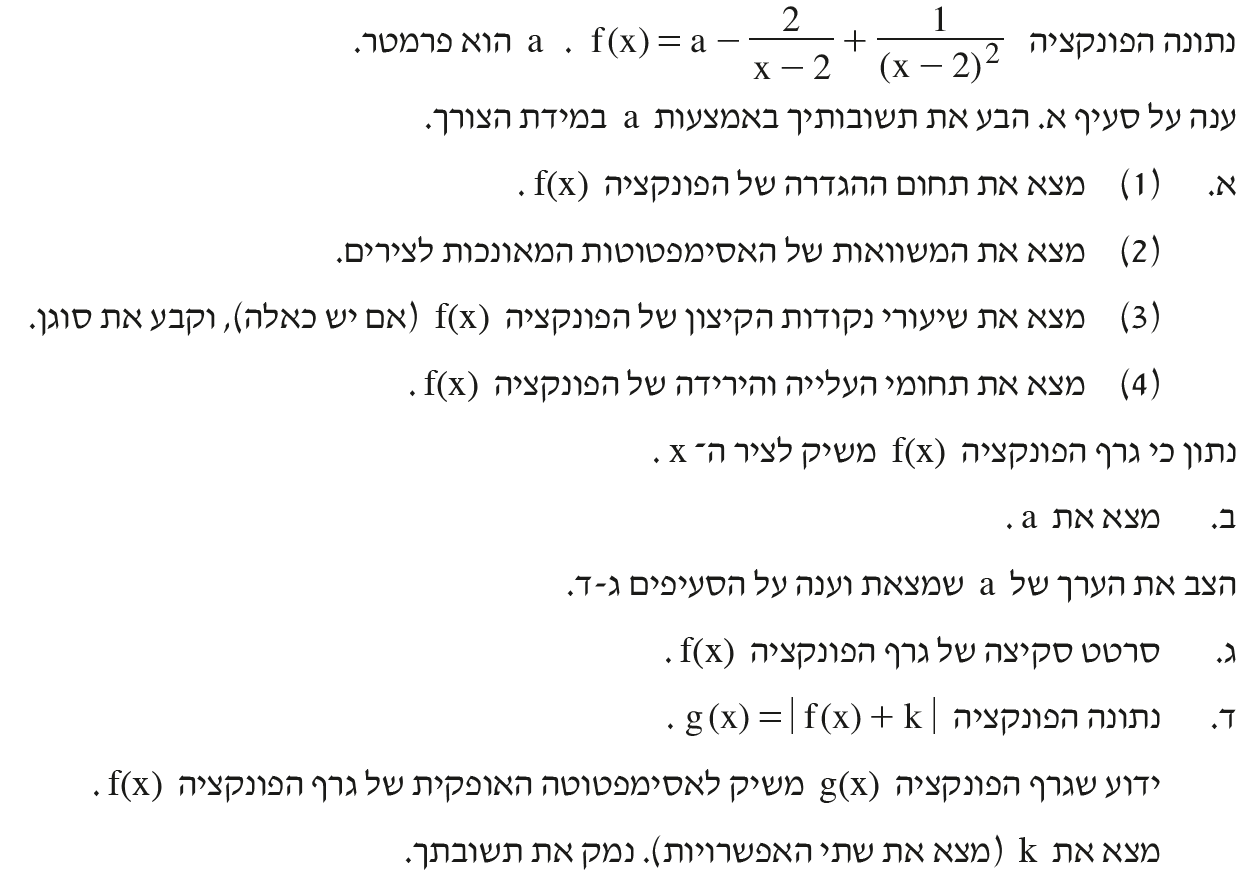
\includegraphics[width=\textwidth]{summer-2017b-6}
\end{center}

\textbf{סעיף א}

$(1)$
תחום ההגדה הוא
$x\neq 2$
כי
$x=2$
מאפס את המכנה של שני גורמים.

$(2)$
כאשר 
$x\rightarrow \pm\infty$
שני גורמים שואפים לאפס, ולכן ה%
\asm{}
האופקית היא
$y=a$.

כאשר 
$x\rightarrow \pm 2$
שני גורמים שואפים לאינסוף, ולכן ה%
\asm{}
האנכית היא
$x=2$.

נבדוק את סימן הפונקציה השואפת לאינסוף. כאשר
$x\rightarrow 2$,
$\frac{1}{(x-2)^2}\gg\frac{2}{x-2}$
כך ש-%
$y\rightarrow+\infty$
גם מימין וגם משמאל.

$(3)$
\[
f'(x) = -\frac{2\cdot -1}{(x-2)^2} + \frac{-2}{(x-2)^3}=0\,.
\]
הפוקציה לא מוגדרת ב-% 
$x=2$,
כך שאפשר להכפיל את המשוואה ב-%
$(x-2)^3$.
נקבל
$2(x-2)=2$
ו-%
$x=3$.
נקודת הקיצון היא
$(3,a-1)$.

על ידי הכפלה ב-% 
$(x-2)$
וב-%
$(x-2)^2$
הנגזרת הראשונה היא:
\[
f'(x) = \frac{2(x-2)^2-2(x-2)}{(x-2)^4}=\frac{2x^2-10x+12)}{(x-2)^4}\,.
\]

\np

המכנה חיובי לכן הסימן של הנגזרת השנייה הוא סימן נגזרת המונה
$4x-10$.
ב-%
$x=3$,
הסימן חיובי והנקודת הקיצון היא מינימום.

דרך אחרת לבדוק אם מדובר במינימום או מקסימום היא באמצעות טבלת עליות וירידות:
\[
\begin{array}{c|c|c|c|c|c}
x & 0 & 2 & 2.5 & 3 & 4\\\hline
f'(x) & 0.75 & \times & -0.5& 0 & 0.25\\\hline
f(x) & \nearrow & \times & \searrow & a-1 & \nearrow
\end{array}
\]
הנקודה
$(3,a-1)$
היא מינימום.

$(4)$
ראו בסעיף הקודם.

\textbf{סעיף ב}

נתון שערכה של
$f(x)$
בנקודת המינימום הוא אפס.
$f(3)=a-1=0$
ו-%
$a=1$.

\textbf{סעיף ג}

לפי טבלת העליות והירידות, הפונקציה עולה עד ל%
\asm{}
האנכית, אח"כ יורדת לנקודת המינימום ואח"כ עולה.

\begin{center}
\selectlanguage{english}
\begin{tikzpicture}[scale=1]
\begin{axis}[
    xlabel = $x$,
    ylabel = {$f(x)$},
    axis lines=center,
    xtick={-2,...,7},
    ytick={-1,...,5},
    xmin = -2,
    xmax = 7,
    ymin = -1,
    ymax = 5,
    xticklabel style={
    anchor=north east,
    },
    yticklabel style={
    anchor=south east,
    },
    every axis y label/.style={at={(ticklabel cs:0.7)},rotate=90,anchor=west,},
    every axis x label/.style={at={(ticklabel cs:0.7)},anchor=north,},
]
\addplot [
    domain=-2:1.3, 
    samples=40, 
]
{1-(2/(x-2))+(1/(x-2)^2)};
\addplot [
    domain=2.3:7, 
    samples=40, 
]
{1-(2/(x-2))+(1/(x-2)^2)};
\draw[dashed,thick] ({axis cs:2,0}|-{rel axis cs:0,0}) -- ({axis cs:2,0}|-{rel axis cs:0,1});
\draw[dashed,thick] ({axis cs:-2,1}-|{rel axis cs:0,0}) -- ({axis cs:-2,1}-|{rel axis cs:7,0});
\fill (axis cs:3,0) circle(1.5pt);
\end{axis}
\end{tikzpicture}
\end{center}


\textbf{סעיף ד}
ה%
\asm{}
האופקית היא
$y=a=1$
ונקודת המינימום היא
$(3,a-1)=(3,0)$:
\begin{eqnarray*}
g(3)&=&|f(3)+k|=a=1\\
|0+k|&=&1\\
k&=&\pm 1\,.
\end{eqnarray*}

%%%%%%%%%%%%%%%%%%%%%%%%%%%%%%%%%%%%%%%%%%%%%%%%%%%%%%%%%%%%%%%%%%%%%%


\section{קיץ תשע"ז מועד א}

\begin{center}
\selectlanguage{english}
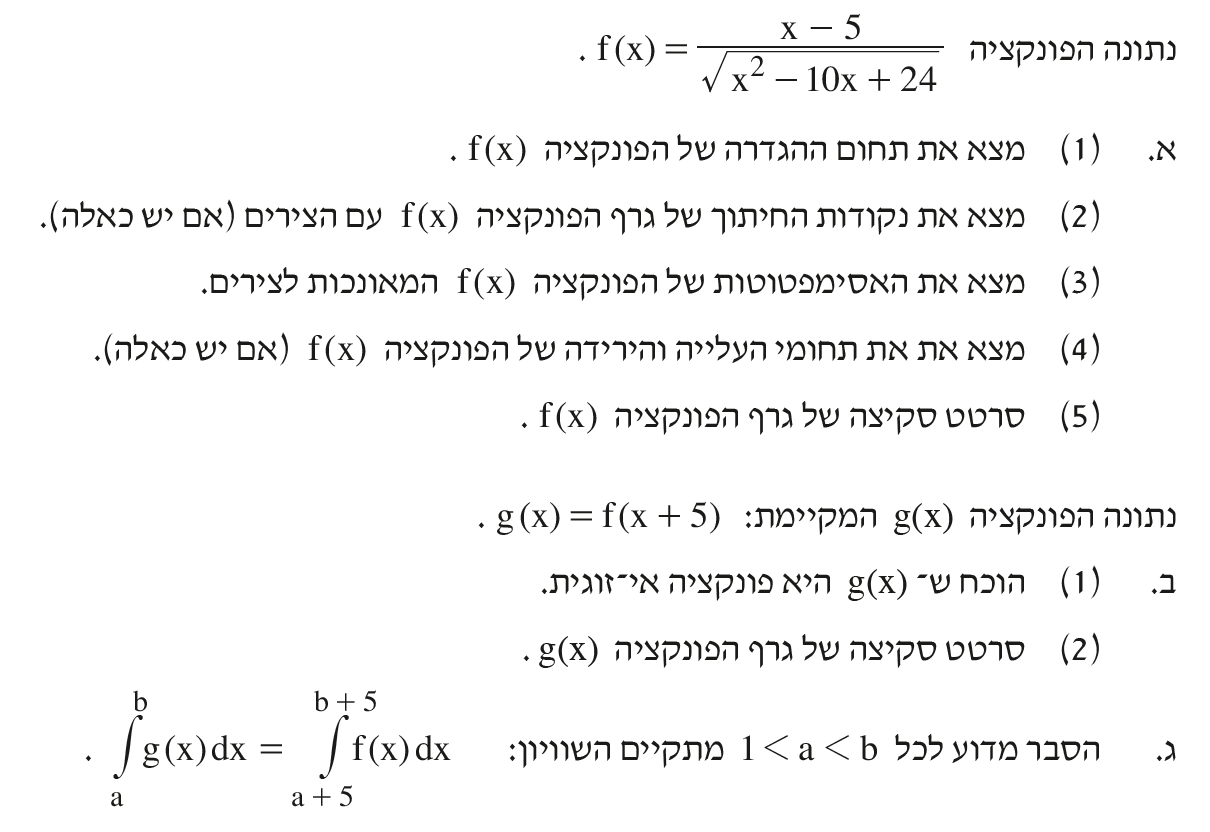
\includegraphics[width=\textwidth]{summer-2017a-6}
\end{center}

\vspace{-5ex}

\textbf{סעיף א}


$(1)$
הפונקציה מוגדרת אם המכנה שונה מאפס ואם הביטוי בשורש גדול או שווה לאפס:
\begin{equationarray*}{rcl}
x^2-10x+24 &>& 0\\
(x-4)(x-6) &>& 0\,.
\end{equationarray*}
המכפלה חיובית רק אם שני הגורמים גדולים מאפס או שניהם קטנים מאפס. אבל אם 
$x>6$
אז 
$x>4$
ואם
$x<4$
אז 
$x<6$,
ולכן הפונקציה מוגדרת כאשר:
\[
x<4 \quad 
\textrm{\R{או}}
\quad x>6\,.
\]
$(2)$
$f(x)=0$
אם המכנה חיובי והמונה 
$x-5=0$.
אבל 
$5$
לא בתחום ההגדרה כך שאין נקודת חיתוך עם ציר ה-%
$x$.
חישוב נקודת החיתוך 
$(0,y)$
עם ציר ה-%
$y$:
\[
y=f(0)=\frac{0-5}{\sqrt{0^2-10\cdot 0 + 24}}=\frac{-5}{\sqrt{24}}\,.
\]
$(3)$
כאשר 
$x\rightarrow 6^{+}$
המונה שואף ל-%
$1$.
המכנה שורש חיובי שהולך וקטן, ולכן
$f(x)\rightarrow +\infty$.
$x=6$
היא
\asm{}
אנכית אחת. באופן דומה, כאשר
$x\rightarrow 4^{-}$,
$f(x)\rightarrow -\infty$,
ו-%
$x=4$
היא
\asm{}
אנכית שנייה.

כאשר 
$x\rightarrow +\infty$
המנה שואף ל-%
$+\infty$.
כאשר 
$x\rightarrow +\infty$,
במכנה
$x^2\gg -10x+24$,
וערכו מתקרב ל-%
$\sqrt{x^2}=x$
שגם הוא שואף ל-%
$+\infty$.
לכן
$y\rightarrow 1$
היא
\asm{}
אופקית אחת. באופן דומה, כאשר
$x\rightarrow -\infty$,
$y\rightarrow -1$
ו-%
$y=-1$
היא
\asm{}
אופקית שנייה.

\np

$(4)$
אי-אפשר פשוט להכין טבלה של עליות וירידות, כי אין אנו יודעים אם יש נקודות קיצון בתחום ההגדרה של הפונקציה. כצעד ראשון נבדוק את ערכו של
$f(x)'$.
לשם קיצור נסמן
$u=x^2-10x+24$.
הנגזרת היא:
\[
\frac{1\cdot \sqrt{u} - (x-5)\cdot \frac{1}{2} u^{-\frac{1}{2}} \cdot (2x-10)}{u}=\frac{u - (x-5)(x-5)}{u\sqrt{u}}\,.
\]
$u$
חיובי
\textbf{בתחום ההגדרה}
וגם
$\sqrt{u}$
חיובי, ולכן הסימן או נקודת האיפוס של הנגזרת תלוי רק במונה:
\[
u-(x-5)(x-5)=x^2-10x+24-x^2+10x-25=-1\,.
\]
בתחום ההגדרה, הנגזרת שלילית )ולא מתאפסת(, ולכן הפונקציה יורדת בכל תחום ההגדרה.

\vspace{1ex}
$(5)$

\vspace{-3ex}

\begin{center}
\selectlanguage{english}
\begin{tikzpicture}[scale=.9]
\begin{axis}[
    xlabel = $x$,
    ylabel = {$f(x)$},
    axis lines=center,
    xtick={-1,...,8},
    ytick={-3,...,3},
    xmin = -1,
    xmax = 8,
    ymin = -3,
    ymax = 3,
    xticklabel style={
    anchor=north east,
    },
    yticklabel style={
    anchor=south east,
    },
    every axis y label/.style={at={(ticklabel cs:0.7)},rotate=90,anchor=west,},
    every axis x label/.style={at={(ticklabel cs:0.7)},anchor=center,},
]
\addplot [
    domain=-1:3.9, 
    samples=40, 
]
{(x-5)/sqrt(x^2-10*x+24)};
\addplot [
    domain=6.1:8, 
    samples=40, 
]
{(x-5)/sqrt(x^2-10*x+24)};
\draw[dashed,thick] ({axis cs:4,-3}|-{rel axis cs:0,0}) -- ({axis cs:4,-3}|-{rel axis cs:0,6});
\draw[dashed,thick] ({axis cs:6,-3}|-{rel axis cs:0,0}) -- ({axis cs:6,-3}|-{rel axis cs:0,6});
\draw[dashed,thick] ({axis cs:-1,1}-|{rel axis cs:0,0}) -- ({axis cs:-1,1}-|{rel axis cs:9,0});
\draw[dashed,thick] ({axis cs:-1,-1}-|{rel axis cs:0,0}) -- ({axis cs:-1,-1}-|{rel axis cs:9,0});
\end{axis}
\end{tikzpicture}
\end{center}

\vspace{-3ex}

\textbf{סעיף ב}

$(1)$
פתרון אחד הוא לחשב את
$g(x),g(-x)$
ולהראות ש-%
$g(-x)=-g(x)$:

\vspace{-4ex}

\erh{11pt}
\begin{equationarray*}{rcl}
g(-x) &=& f(-x+5)=f(5-x)\\
&=& \frac{5-x-5}{\sqrt{(5-x)^2-10(5-x)+24}}\\
&=&\frac{-x}{\sqrt{25-10x+x^2-50+10x+24}}\\
&=&\frac{-x}{\sqrt{x^2-1}}\,,
\end{equationarray*}

\vspace{-7ex}

\erh{11pt}
\begin{equationarray*}{rcl}
g(x) &=& f(x+5)\\
&=& \frac{x+5-5}{\sqrt{(x+5)^2-10(x+5)+24}}\\
&=&\frac{x}{\sqrt{x^2+10x+25-10x-50+24}}\\
&=&\frac{x}{\sqrt{x^2-1}}\,.
\end{equationarray*}

\vspace{-3ex}

\np

פתרון מעט יותר מסובך הוא להראות
$g(-x)=-g(x)$
בצורה ישירה:
\erh{12pt}
\begin{equationarray*}{rcl}
g(-x) &=& f(-x+5)=f(5-x)\\
&=& \frac{5-x-5}{\sqrt{(5-x)^2-10(5-x)+24}}\\
&=&\frac{-x}{\sqrt{25-10x+x^2-50+10x+24}}\\
&=&\frac{-x}{\sqrt{x^2+10x+25-10x-50+24}}\\
&=&\frac{-((x+5)-5)}{\sqrt{(x+5)^2-10(x+5)+24}}\\
&=&-g(x)\,.
\end{equationarray*}

\vspace{-3ex}

$(2)$
הגרף הוא אותו גרף מוזז שמאלה חמש יחידות:

\begin{center}
\selectlanguage{english}
\begin{tikzpicture}[scale=.9]
\begin{axis}[
    xlabel = $x$,
    ylabel = {$f(x)$},
    axis lines=center,
    xtick={-6,...,3},
    ytick={-3,...,3},
    xmin = -6,
    xmax = 3,
    ymin = -3,
    ymax = 3,
    xticklabel style={
    anchor=north east,
    },
    yticklabel style={
    anchor=south east,
    },
    every axis y label/.style={at={(ticklabel cs:0.8)},rotate=90,anchor=south,},
    every axis x label/.style={at={(ticklabel cs:0.9)},anchor=center,},
]
\addplot [
    domain=-6:-1.1, 
    samples=40, 
]
{x/sqrt((x+5)^2-10*(x+5)+24)};
\addplot [
    domain=1.1:3, 
    samples=40, 
]
{x/sqrt((x+5)^2-10*(x+5)+24)};
\draw[dashed,thick] ({axis cs:-1,-3}|-{rel axis cs:0,0}) -- ({axis cs:-1,-3}|-{rel axis cs:0,6});
\draw[dashed,thick] ({axis cs:1,-3}|-{rel axis cs:0,0}) -- ({axis cs:1,-3}|-{rel axis cs:0,6});
\draw[dashed,thick] ({axis cs:-6,1}-|{rel axis cs:0,0}) -- ({axis cs:-6,1}-|{rel axis cs:9,0});
\draw[dashed,thick] ({axis cs:-6,-1}-|{rel axis cs:0,0}) -- ({axis cs:-6,-1}-|{rel axis cs:9,0});
\end{axis}
\end{tikzpicture}
\end{center}

\textbf{סעיף ג}

נתון ש-%
$1<a<b$,
וכפי שניתן לראות מהגרף,
$a,b$
הם בתחום ההגדרה של 
$g$.
נחשב:
\[
\int_a^b g(x) dx = \int_a^b f(x+5) dx = \int_{a+5}^{b+5} f(x) dx\,.
\]


%%%%%%%%%%%%%%%%%%%%%%%%%%%%%%%%%%%%%%%%%%%%%%%%%%%%%%%%%%%%%%%%%%%%%%


\section{חורף תשע"ז}

\begin{center}
\selectlanguage{english}
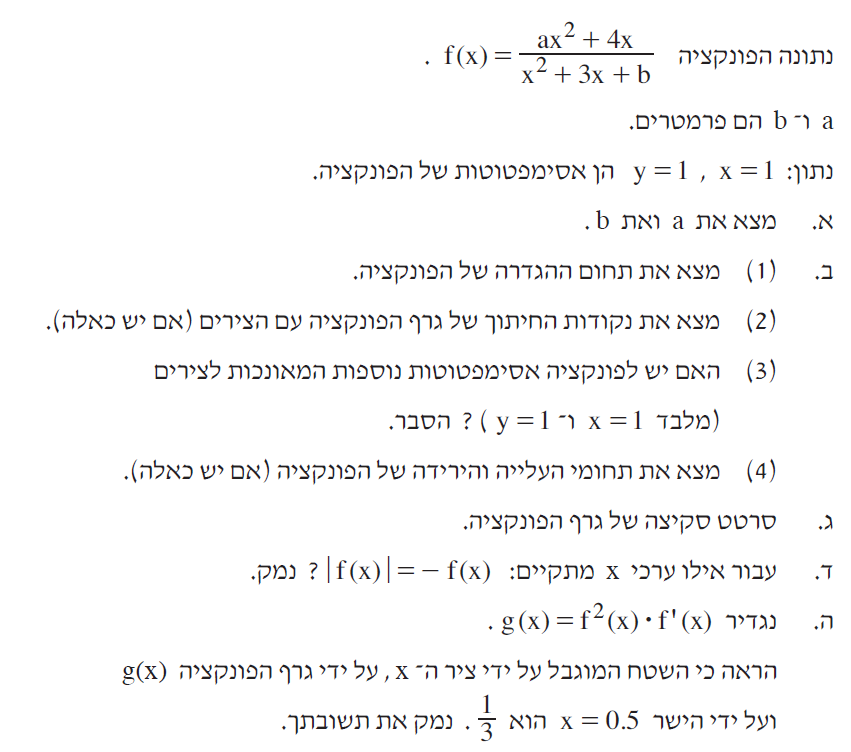
\includegraphics[width=\textwidth]{winter-2017-6}
\end{center}

\vspace{-3ex}

\textbf{סעיף א}

נקבל את ה%
\asm{}
אנכית
$x=1$
כאשר המכנה שווה לאפס עבור ערך זה:
\erh{0pt}
\begin{equationarray*}{rcl}
x^2+3x+b&=&0\\
1^2+3\cdot 1+b&=&0\\
b&=&-4\,.
\end{equationarray*}
נחשב את ה%
\asm{}
האופקית
$y=1$.
כאשר 
$x\rightarrow 1$:
\[
\frac{a+\frac{4}{x}}{1+\frac{3}{x}-\frac{4}{x^2}} \rightarrow 1\,,
\]
ו-%
$a=1$.

\textbf{סעיף ב}

$(1)$
נבדוק מתי המכנה מתאפס:
\[
x^2+3x-4=(x+4)(x-1)\,,
\]
ולכן הפונקציה מוגדרת עבור כל 
$x$
פרט ל-%
$x=1,x=-4$.

\np

$(2)$
נציב 
$x=0$.
המונה מתאפס והמכנה לא מתאפס ולכן נקודת החיתוך עם ציר ה-%
$y$
היא
$(0,0)$.

נציב 
$y=0$
ונקבל
$x^2+4x=x(x+4)=0$.
$(0,0)$
היא נקודת חיתוך עם שני הצירים. ב-%
$x=-4$
הפונקציה לא מוגדרת, ולכן אין עוד נקודת חיתוך עם ציר ה-%
$x$.


$(3)$
אין עוד 
\asm{} 
אופקיות כי לפי החישוב בסעיף א, ה-%
\asm{}
היא
$\frac{a}{1}$ 
שיש לה רק פתרון אחד כי 
$a$
הוא קבוע.

\asm{}
אנכית יש כאשר 
$x^2+3x-4=(x+4)(x-1)=0$.
אבל 
$x=-4$
גם מאפס את המונה. נצמצם את הפונקציה:
\[
\frac{x^2+4x}{x^2+3x-4}=\frac{x(x+4)}{(x+4)(x-1)}=\frac{x}{x-1}\,.
\]
כאשר 
$x\rightarrow -4$
)בשני הכיוונים(, ערך הפונקציה שואפת ל-%
$\frac{4}{5}$,
ולכן אין כאן
\asm{} 
אלא חור.

$(4)$
נחשב את הנגזרת, כאשר נתייחס רק למונה כי המכנה הוא ריבוע שתמיד חיובי פרט לנקודות של החור וה%
\asm{}:
\[
(x^2+4x)'(x^2+3x-4)-(x^2+4x)(x^2+3x-4)'=-(x+4)^2\,.
\]
)לא רשמתי את כל החישובים הארוכים.( ערך זה לא מתאפס ותמיד שלילי, ולכן הפונקציה יורדת בכל תחום ההגדרה שלה.

אפשר לקצר אם נצמצם את הפונקציה לפי נמחשב את הנגזרת. 
$\left(\frac{x}{x-1}\right)'=-1$,
שתמיד שלילי.

\textbf{סעיף ג}
\begin{center}
\selectlanguage{english}
\begin{tikzpicture}[scale=1]
\begin{axis}[
    xlabel = $x$,
    ylabel = {$f(x)$},
    axis lines=center,
    xtick={-6,...,5},
    ytick={-3,...,3},
    xmin = -6,
    xmax = 5,
    ymin = -3,
    ymax = 3,
    every axis y label/.style={at={(ticklabel cs:0.8)},rotate=90,anchor=west,},
    every axis x label/.style={at={(ticklabel cs:0.9)},anchor=north,},
]
\addplot [
    domain=-6:-4.05, 
    samples=40, 
]
{(x^2+4*x)/(x^2+3*x-4)};
\addplot [
    domain=-3.95:.9, 
    samples=40, 
]
{(x^2+4*x)/(x^2+3*x-4)};
\addplot [
    domain=1.1:4, 
    samples=40, 
]
{(x^2+4*x)/(x^2+3*x-4)};
\draw[dashed,thick] ({axis cs:-6,1}-|{rel axis cs:0,0}) -- ({axis cs:-6,1}-|{rel axis cs:11,0});
\draw[dashed,thick] ({axis cs:1,-3}|-{rel axis cs:0,0}) -- ({axis cs:1,-3}|-{rel axis cs:0,6});
\fill (axis cs:0,0) circle(1.5pt);
\draw (axis cs:-4,.8) circle(1.5pt);
\end{axis}
\end{tikzpicture}
\end{center}

\textbf{סעיף ד}

אם נתייחס לגרף, 
$|f(x)|$
מעביר ערכים מתחת לציר ה-%
$x$
לערכים מעל לציר, ו-%
$-f(x)$
מעביר את כל הערכים לצד השני של ציר ה-%
$x$.
$|f(x)|=-f(x)$
רק עבור ערכים מתחת לציר ה-%
$x$
כי רק עבור ערכים אלה שניהם מבצעים אותה פעולה. עבור פונקציה זו הערכים הם
$0\leq x < 1$.

\textbf{סעיף ה}

מסעיף ב 
$f'(x)$
תמיד שלילי ולכן
$g(x)=f(x)^2\cdot f'(x)$
תמיד שלילי או אפס. ראינו גם ש-%
$f(0)=0$,
ולכן השטח שיש לחשב נמצא מתחת לציר ה-%
$x$
ומימין לציר ה-%
$y$.

\np

\begin{center}
\selectlanguage{english}
\begin{tikzpicture}[scale=.8]
\begin{axis}[
    axis lines=center,
    xtick={-.5,.5,1},
    ytick={0},
    xmin = -.5,
    xmax = 1,
    ymin = -1.1,
    ymax = .5,
]
\addplot [
    domain=0:.6, 
    samples=40,
]
{(x^2+4*x)/(x^2+3*x-4)};
\draw ({axis cs:.5,-1}|-{rel axis cs:0,0}) -- ({axis cs:.5,-1}|-{rel axis cs:0,1});
\end{axis}
\end{tikzpicture}
\end{center}
)התרשים לא מדוייק.(

נשים לב ש-%
$(f^3(x))'=3f^2(x)\cdot f'(x)$,
ונוכל לחשב את האינטגרל:
\[
\int_0^{0.5} 0-f^2(x)\cdot f'(x)=\left.-\frac{1}{3}f^3(x)\right|^{0.5}_0=-\frac{1}{3}f^3(0.5)\,.
\]
כי 
$f(0)=0$.

\[
f(0.5)=\frac{0.25+2}{0.25+1.5-4}=-1\,,
\]
והשטח הוא:
\[
-\frac{1}{3}f^3(0.5)=-\frac{1}{3}\cdot (-1)^3=\frac{1}{3}\,.
\]

\end{comment}

%%%%%%%%%%%%%%%%%%%%%%%%%%%%%%%%%%%%%%%%%%%%%%%%%%%%%%%%%%%%%%%%%%%%%%

\section{קיץ תשע"ו מועד ב}

\begin{center}
\selectlanguage{english}
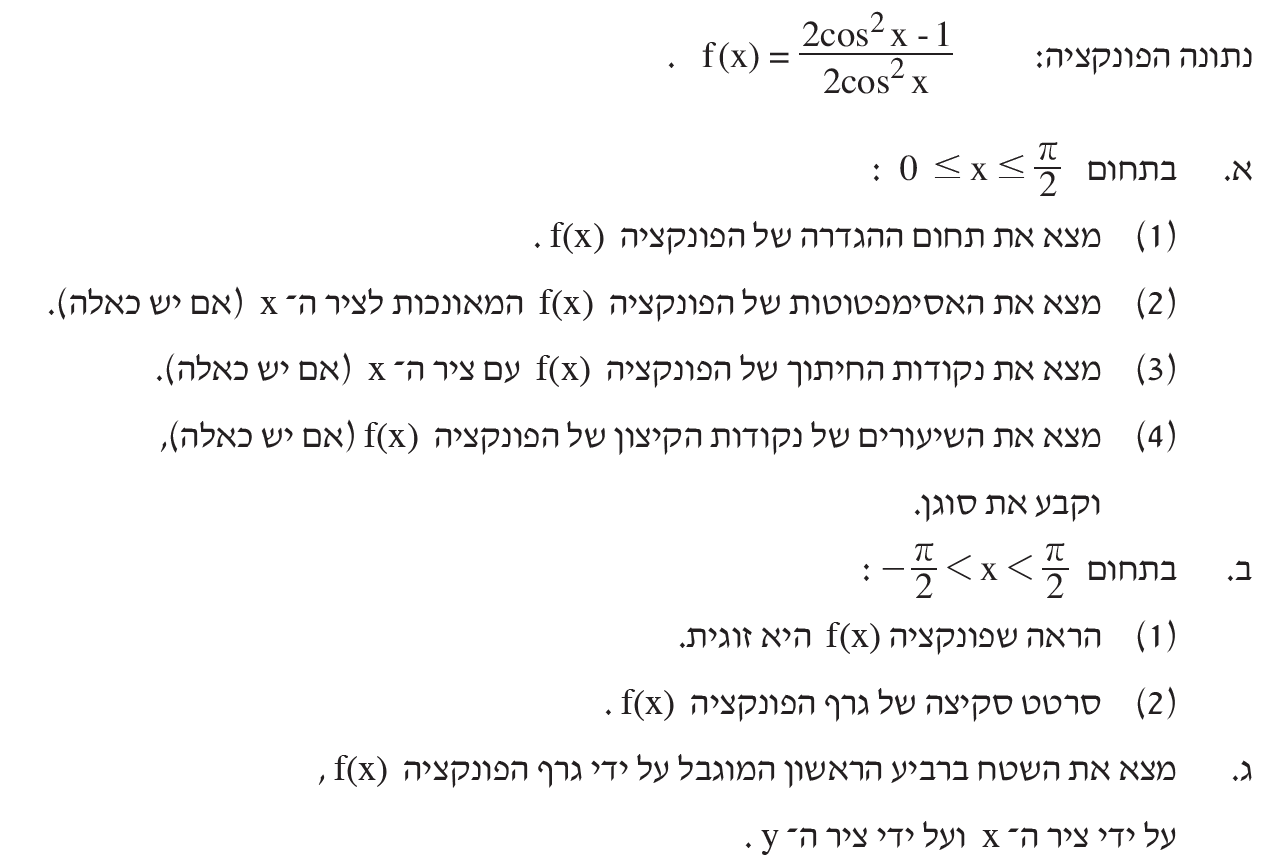
\includegraphics[width=\textwidth]{summer-2016b-6}
\end{center}

\textbf{סעיף א}

$(1)$
הפונקציה לא מוגדרת כאשר המכנה מתאפס.
$\cos^2 x=0$
בתחום כאשר
$x=\frac{\pi}{2}$,
ולכן תחום ההגדרה הוא
$0\leq x< \frac{\pi}{2}$.

$(2)$
כאשר
$x\rightarrow \frac{\pi}{2}$,
המכנה שואף לאפס אבל המונה שואף לערך שונה מאפס
$-1$,
ולכן
$x=\frac{\pi}{2}$
היא
\asm{}
אנכית.

$(3)$
בתחום ההגדרה המכנה לא מאפס, ולכן נקודות החיתוך הן הנקודות עבורן המונה מתאפס:
\erh{6pt}
\begin{equationarray*}{rcl}
2\cos^2 x &=& 1\\
\cos x &=& \frac{1}{\sqrt{2}}=\frac{\sqrt{2}}{2}\,.
\end{equationarray*}
בתחום ההגדרה יש רק פתרון אחד ונקודת הקיצון הוא
$(\frac{\pi}{4},0)$.


$(4)$
בתחום ההגדרה המכנה לא מתאפס ולכן ניתון לצמצם את הפונקציה כדי להקל על חישוב הנגרת:
\[
f'(x)=\left(-\frac{1}{\cos^2 x}\right)'=-\left(-2\cos x \cdot -\sin x\right)=-2\cos x \sin x = 0\,.
\]
$f'(x)$
מתאפס בתחום ההגדרה כאשר 
$\sin x = 0$,
$x = 0$,
ונקודת הקיצון היא
$(0,\frac{1}{2})$.
בתחום ההגדרה סינוס וקוסינוס חיוביים, הנגזרת שלילית, הפונקציה יורדת ונקודת הקיצון הוא מקסימום.
\np

\textbf{סעיף ב}

$(1)$

$\cos(-x)=\cos x$,
$\cos^2(-x)=\cos^2 x$
והפונקציה זוגית.


$(2)$
המקסימום הוא ב-%
$(0,\frac{1}{2})$,
הפונקציה יורדת בתחום ההגדרה, יש 
\asm{}
אנכית ב-%
$\frac{\pi}{2}$,
והפונקציה זוגית. התרשים שמתקבל הוא:
\begin{center}
\selectlanguage{english}
\begin{tikzpicture}%[scale=.9]
\begin{axis}[
    trig format plots=rad,
    axis lines=center,
    xmin=-1.65,
    xmax=1.6,
    xtick={-1.57,-.785,0,.785,1.57},
    xticklabels={$\quad\quad -\frac{\pi}{2}$,$\;\;-\frac{\pi}{4}$,$0$,
                 $\!\!\frac{\pi}{4}$,$\quad\frac{\pi}{2}$},
    ymin = -2,
    ymax = 1.5,
    ymajorticks=false,
    xticklabel style={anchor=north,},
]
\addplot [
    domain=-1.5:1.5, 
    samples=40, 
]
{(2*(cos(x))^2-1)/(2*(cos(x))^2)};
\draw[dashed,thick] (axis cs:-1.57,-2) -- (axis cs:-1.57,1.5);
\draw[dashed,thick] (axis cs:1.57,-2) -- (axis cs:1.57,1.5);
\fill (axis cs:0,.5) circle(1.5pt);
\fill (axis cs:-.785,0) circle(1.5pt);
\fill (axis cs:.785,0) circle(1.5pt);
\node at (axis cs:.15,.75) {$\frac{1}{2}$};
\end{axis}
\end{tikzpicture}
\end{center}



\textbf{סעיף ג}

הנוסחה
$(\tan x)'=\frac{1}{\cos^2 x}$
אמנם מופיעה בנוסחאון אבל לא מרבים להשתמש בה, כך שהשאלה עלולה להיות קשה.
\erh{14pt}
\begin{equationarray*}{rcl}
\int_0^{\frac{\pi}{4}} \frac{2\cos^2 x -1}{2\cos^2 x}&=&\int_0^{\frac{\pi}{4}} 1 - \int_0^{\frac{\pi}{4}}\frac{1}{2\cos^2 x}\\
&=&\left.x\right|_0^{\frac{\pi}{4}} - \left.\frac{1}{2}\tan x\right|_0^{\frac{\pi}{4}}\\
&=&\frac{\pi}{4}-0-\frac{1}{2}\tan \frac{\pi}{4} + \frac{1}{2}\tan 0=\frac{\pi}{4}-\frac{1}{2}\,.
\end{equationarray*}

\begin{comment}



%%%%%%%%%%%%%%%%%%%%%%%%%%%%%%%%%%%%%%%%%%%%%%%%%%%%%%%%%%%%%%%%%%%%%%

\section{קיץ תשע"ה מועד ב}

\begin{center}
\selectlanguage{english}
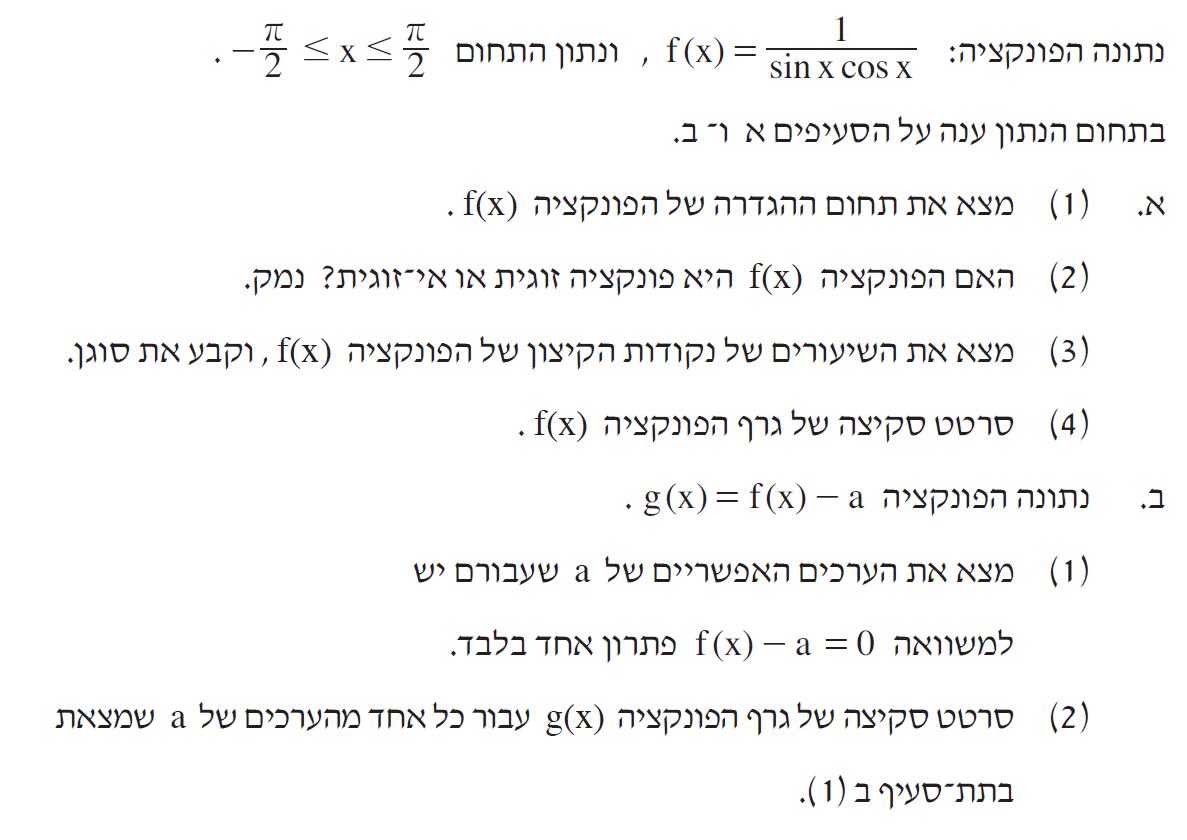
\includegraphics[width=\textwidth]{summer-2015b-6}
\end{center}

\textbf{סעיף א}

$(1)$
ערך הוא מחוץ לתחום ההגדרה כאשר הוא מאפס את המכנה. 
$\sin 0=0$, $\cos \frac{\pi}{2}= \cos -\frac{\pi}{2}=0$ 
ותחום ההגדרה הוא:
\[
-\frac{\pi}{2} < x < 0,\quad 0 < x < \frac{\pi}{2}\,.
\]

$(2)$
הפונקציה סינוס היא אי-זוגית והפונקציה קוסינוס היא זוגית. המכפלה שלהן היא אי-זוגיות.

$(3)$
\[
((\sin x \cos x)^{-1})'= -1\cdot (\sin x \cos x)^{-2}(\sin x\cos x)'\,.
\]
בתחום ההגדרה המכנה חיובי, כך שנאשר רק לבדוק אם המונה יכול להתאפס.
\[
-(\sin x\cos x)'=-(\cos^2 x-\sin^2 x)=(\sin^2 x-\cos^2 x)=0\,.
\]
נקודות הקיצון הן בערכים שיש להם ערך מוחלט של סינוס שווה לערך מוחלט של קוסינוס, שהם כפולות של 
$\frac{\pi}{4}$.
בתחום ההגדרה:
\[
x=\pm\frac{\pi}{4},\quad y=\frac{2\cdot 2}{\pm\sqrt{2}\cdot\sqrt{2}}=\pm 2\,.
\]

\np

המכנה של הנגזרת הראשונה הוא 
$(\sin x \cos x)^2$,
ערך חיובי בתחום ההגדרה, ולכן, סימן הנגזרת השנייה הוא כסימן הנגזרת של המונה.
\[
(\sin^2 x-\cos^2 x)'=2\sin x \cos x -2 \cos x (-\sin x)=4\sin x\cos x\,.
\]
עבור
$x=\frac{\pi}{4}$,
$4\sin x\cos x=2<0$
והנקודה היא מינימום.

עבור
$x=-\frac{\pi}{4}$,
$4\sin x\cos x=-2<0$
והנקודה היא מקסימום.

$(4)$
\begin{center}
\selectlanguage{english}
\begin{tikzpicture}[scale=.9]
\begin{axis}[
    trig format plots=rad,
    axis lines=center,
    xmin=-1.57,
    xmax=1.57,
    xtick={-1.57,-.785,0,.785,1.57},
    xticklabels={$-\frac{\pi}{2}$,$-\frac{\pi}{4}$,$0$,
                 $\frac{\pi}{4}$,$\frac{\pi}{2}$},
    ymin = -4,
    ymax = 4,
    ytick={-2,2},
    yticklabels={$-2$,$2$},
    xticklabel style={anchor=north east,},
]
\addplot [
    domain=-1.55:-.05, 
    samples=40, 
]
{1/(sin(x)*cos(x))};
\addplot [
    domain=.05:1.55, 
    samples=40, 
]
{1/(sin(x)*cos(x))};
\draw[dashed,thick] ({axis cs:-1.57,-4}|-{rel axis cs:0,0}) -- ({axis cs:-1.57,-4}|-{rel axis cs:0,3.14});
\draw[dashed,thick] ({axis cs:1.57,-4}|-{rel axis cs:0,0}) -- ({axis cs:1.57,-4}|-{rel axis cs:0,3.14});
\fill (axis cs:.785,2) circle(1.5pt);
\fill (axis cs:-.785,-2) circle(1.5pt);
\end{axis}
\end{tikzpicture}
\end{center}

\textbf{סעיף ב}

$(1)$
למשוואה פתרון אחד אם הגרף משיק לציר ה-%
$x$
או חותך את הציר במקום אחד בלבד. מצב זה מתקבל כאשר 
$a=\pm 2$
שמעלה או מוריד את הגרף בשתי יחידות.

\begin{center}
\selectlanguage{english}
\begin{tikzpicture}[scale=.9]
\begin{axis}[
    trig format plots=rad,
    axis lines=center,
    xmin=-1.57,
    xmax=1.57,
    xtick={-1.57,-.785,0,.785,1.57},
    xticklabels={$-\frac{\pi}{2}$,$-\frac{\pi}{4}$,$0$,
                 $\frac{\pi}{4}$,$\frac{\pi}{2}$},
    ymin = -6,
    ymax = 6,
    ytick={-2,2},
    yticklabels={$-2$,$2$},
    xticklabel style={anchor=north east,},
]
\addplot [
    domain=-1.55:-.05, 
    samples=40, 
]
{(1/(sin(x)*cos(x)))-2};
\addplot [
    domain=.05:1.55, 
    samples=40, 
]
{(1/(sin(x)*cos(x)))-2};
\draw[dashed,thick] ({axis cs:-1.57,-4}|-{rel axis cs:0,0}) -- ({axis cs:-1.57,-4}|-{rel axis cs:0,3.14});
\draw[dashed,thick] ({axis cs:1.57,-4}|-{rel axis cs:0,0}) -- ({axis cs:1.57,-4}|-{rel axis cs:0,3.14});
\fill (axis cs:.785,0) circle(1.5pt);
\fill (axis cs:-.785,-4) circle(1.5pt);
\end{axis}
\end{tikzpicture}
\hspace{2em}
\begin{tikzpicture}[scale=.9]
\begin{axis}[
    trig format plots=rad,
    axis lines=center,
    xmin=-1.57,
    xmax=1.57,
    xtick={-1.57,-.785,0,.785,1.57},
    xticklabels={$-\frac{\pi}{2}$,$-\frac{\pi}{4}$,$0$,
                 $\frac{\pi}{4}$,$\frac{\pi}{2}$},
    ymin = -6,
    ymax = 6,
    ytick={-2,2},
    yticklabels={$-2$,$2$},
    xticklabel style={anchor=north east,},
]
\addplot [
    domain=-1.55:-.05, 
    samples=40, 
]
{(1/(sin(x)*cos(x)))+2};
\addplot [
    domain=.05:1.55, 
    samples=40, 
]
{(1/(sin(x)*cos(x)))+2};
\draw[dashed,thick] ({axis cs:-1.57,-4}|-{rel axis cs:0,0}) -- ({axis cs:-1.57,-4}|-{rel axis cs:0,3.14});
\draw[dashed,thick] ({axis cs:1.57,-4}|-{rel axis cs:0,0}) -- ({axis cs:1.57,-4}|-{rel axis cs:0,3.14});
\fill (axis cs:.785,4) circle(1.5pt);
\fill (axis cs:-.785,0) circle(1.5pt);
\end{axis}
\end{tikzpicture}
\end{center}



%%%%%%%%%%%%%%%%%%%%%%%%%%%%%%%%%%%%%%%%%%%%%%%%%%%%%%%%%%%%%%%%%%%%%%


\section{קיץ תשע"ה מועד א}

\begin{center}
\selectlanguage{english}
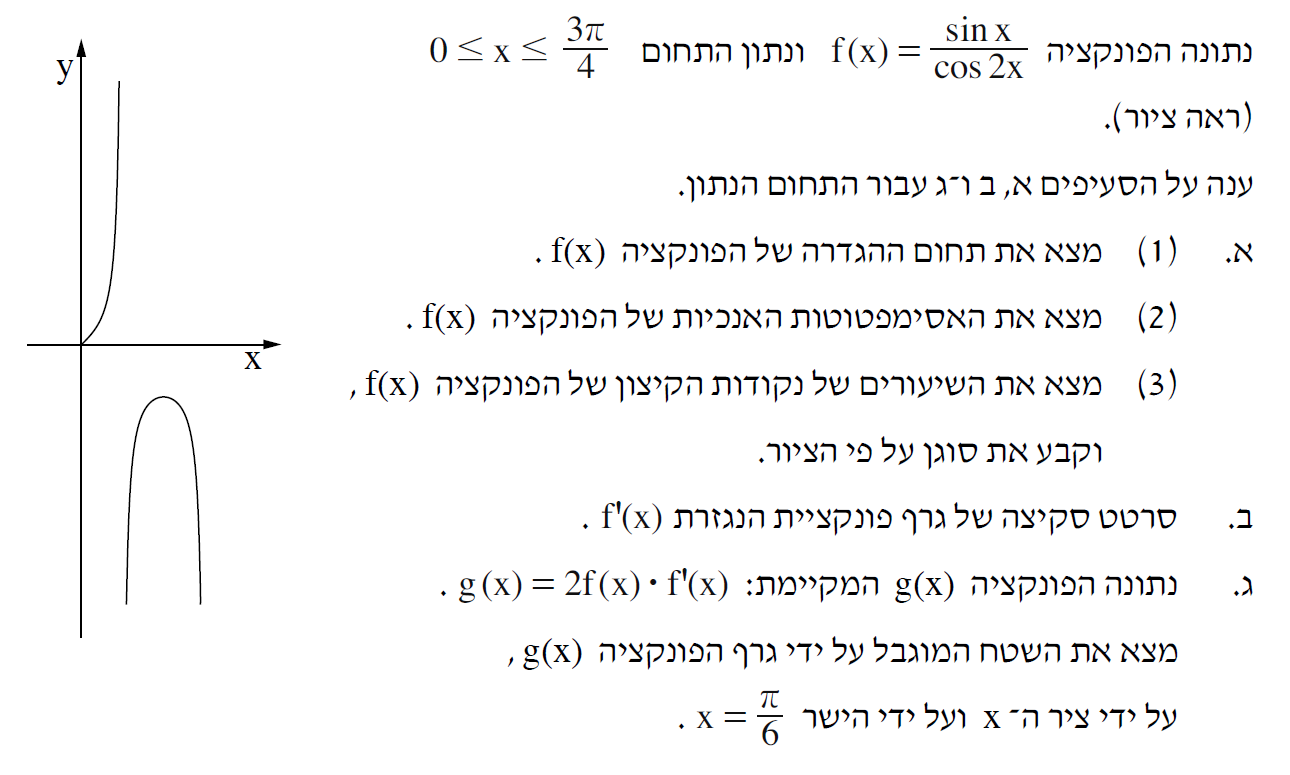
\includegraphics[width=\textwidth]{summer-2015a-6}
\end{center}

\vspace{-4ex}

\textbf{סעיף א}

$(1)$
הפונקציה לא מוגדרת כאשר המכנה מתאפס.
$\cos 2x=0$
כאשר 
$2x=\disfrac{\pi}{2}+k\pi$.
בתרשים להלן רואים שזה קורה עבור
$\disfrac{\pi}{4}, \disfrac{3\pi}{4}$.
תחום ההגדרה הוא:
\[
0\leq x < \disfrac{\pi}{4}, \quad \disfrac{\pi}{4} < x < \disfrac{3\pi}{4}\,.
\]

\vspace{-4ex}

\begin{center}
\selectlanguage{english}
\begin{tikzpicture}
\coordinate (O) at (0,0);
\coordinate (A) at (2,0);
\node[draw,circle through=(A)] at (O) {};
\draw (-2,0) -- (2,0);
\draw (0,-2) -- (0,2);
\draw[ultra thick] (A) arc[start angle=0,end angle=135,radius=2];
\node[right] at (2,0) {$0$};
\fill ($(O)+(45:2)$) circle(3pt) node[above right] {$\disfrac{\pi}{4}$};
\fill ($(O)+(90:2)$) circle(3pt) node[above,yshift=4pt] {$2\cdot\disfrac{\pi}{4}=\disfrac{\pi}{2}+0\cdot \pi$};
\draw[fill] ($(O)+(135:2)$) rectangle +(6pt,6pt) node[left,xshift=-6pt] {$\disfrac{3\pi}{4}$};
\draw[fill] ($(O)+(-90:2)+(-3pt,-3pt)$) rectangle +(6pt,6pt) node[below,yshift=-6pt] {$2\cdot\disfrac{3\pi}{4}=\disfrac{\pi}{2}+1\cdot \pi$};
\end{tikzpicture}
\end{center}

$(2)$
ה%
\asms{} 
הן בערכי ציר ה-%
$x$
בהם הפונקציה לא מוגדרת:
$x=\disfrac{\pi}{4}$, $x=\disfrac{3\pi}{4}$.

$(3)$
יש נקודת קיצון בקצה התחום 
$(0,0)$.
נחשב את הנגזרת כדי לחפש נקודות קיצון פנימיות:

\np

\[
\left(\frac{\sin x}{\cos 2x}\right)'=\frac{\cos x\cos 2x - \sin x (-2\sin 2x)}{\cos^2 2x}\,.
\]
בתחום ההגדרה המכנה חיובי כך הנגזרת תתאפס אם המונה יתאפס.
\begin{equationarray*}{rcl}
\cos x\cos 2x + 2\sin x \sin 2x &=& \cos x(\cos^2x - \sin^2x)+2\sin x\cdot 2\sin x\cos x\\
&=&\cos x(\cos^2x - \sin^2x +4\sin^2 x)\\
&=&\cos x((\cos^2x +\sin^2 x)+2\sin^2x)\\
&=&\cos x(1+2\sin^2 x)\,.
\end{equationarray*}
)אין צורך לזכור את הביטויים עבוד
$\sin 2x$, $\cos 2x$
כי אפשר לשחזר אותם מיידית על ידי חישוב
$\sin (x+x)$, $\cos (x+x)$
לפי הוסחה המופיעה בנוסחאון.(

בתחום ההגדרה
$\cos x$
מתאפס כאשר 
$x=\disfrac{\pi}{2}$,
ו-%
$1+2\sin^2 x$
אף פעם לא מתאפס. נקודת הקיצון היא
$(\disfrac{\pi}{2},-1)$.
לפי הציור מדובר במקסימום מקומי.

\textbf{סעיף ב}
\[
f'(x)=\disfrac{\cos x(1+2\sin^2 x)}{\cos^2 2x}\,.
\]
קל לחשב ש-%
$f'(0)=1$.
בסעיף הקודם חישבנו ש-%
$f'\left(\disfrac{\pi}{2}\right) = 0$.
לפי המכנה
$f'\left(\disfrac{\pi}{4}\right)$
לא מוגדר. בתרשים הנתון ל-%
$f(x)$
רואים שהפונקציה עולה בין
$0$
ל-%
$\disfrac{\pi}{4}$,
ושהנגזרת יורדת בין
$\disfrac{\pi}{4}$
ל-%
$\disfrac{3\pi}{4}$.
התרשים ל-%
$f'(x)$
נראה כך:
\begin{center}
\selectlanguage{english}
\begin{tikzpicture}[scale=.9]
\begin{axis}[
    trig format plots=rad,
    axis lines=center,
    xmin=0,
    xmax=4.71,
    xtick={0,.785,1.57,2.356},
    xticklabels={0,$\disfrac{\pi}{4}$,$\disfrac{\pi}{2}$,$\disfrac{3\pi}{4}$},
    ytick={-4,...,4},
    ymin = -4,
    ymax = 4,
    xticklabel style={anchor=north east,},
]
\addplot [
    domain=0:.72,
    samples=40, 
]
{(cos(x)*(1+2*(sin(x))^2))/(cos(2*x))^2};
\addplot [
    domain=.9:2.1, 
    samples=40, 
]
{(cos(x)*(1+2*(sin(x))^2))/(cos(2*x))^2};
\draw[dashed,thick] ({axis cs:.785,-4}|-{rel axis cs:0,0}) -- ({axis cs:.785,-4}|-{rel axis cs:0,8});
\end{axis}
\end{tikzpicture}
\end{center}

\textbf{סעיף ג}

יש כאן מתנה שיכולה להיות גם מלכודת. המלכודת היא לנסות לחשב את האינטגרל על ידי חישוב הביטוי
$2f(x)\cdot f'(x)$
מהביטויים המפורשים שחישבנו. המתנה היא שאין כל צורך בחישוב כי האיטגרל של
$2f(x)\cdot f'(x)$ 
הוא
$f^2(x)$.
\[
\int_0^{\pi/6} g(x) = f^2(x) \mid_0^{\pi/6}=\frac{\sin (\pi/6)}{\cos (2\pi/6)}-\frac{\sin 0}{\cos 0}=\frac{1/2}{1/2}-\frac{0}{1}=1\,.
\]




%%%%%%%%%%%%%%%%%%%%%%%%%%%%%%%%%%%%%%%%%%%%%%%%%%%%%%%%%%%%%%%%%%%%%%


\section{חורף תשע"ה}

\begin{center}
\selectlanguage{english}
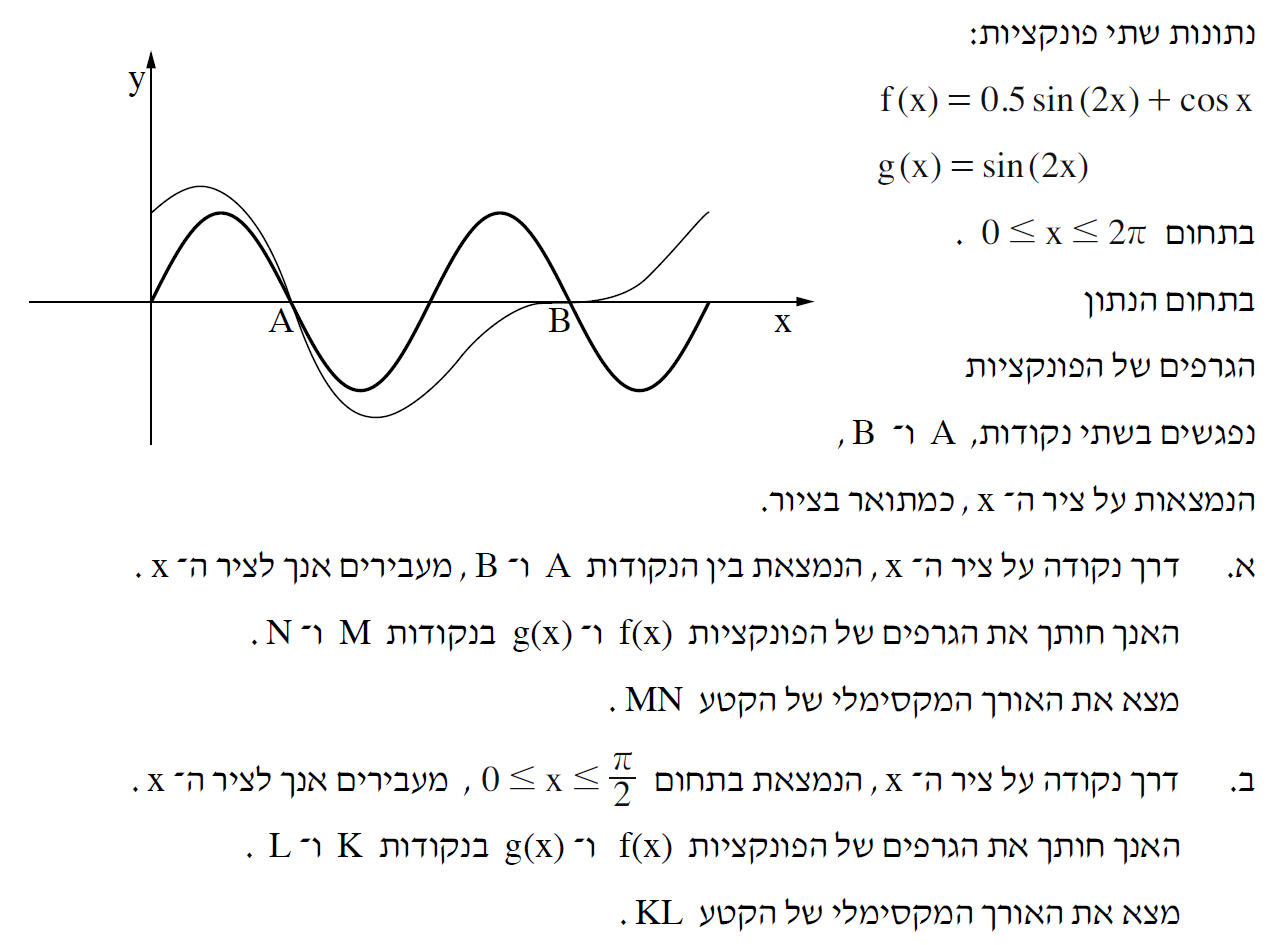
\includegraphics[width=\textwidth]{winter-2015-6}
\end{center}

\vspace{-4ex}


\begin{center}
\selectlanguage{english}
\begin{tikzpicture}%[scale=.9]
\begin{axis}[
    trig format plots=rad,
    axis lines=center,
    xmin=-0,
    xmax=6.283,
    xtick={0,1.57,3.14,4.71,6.283},
    xticklabels={0,$\disfrac{\pi}{2}$,$\pi\:$,$\disfrac{3\pi}{2}\!\!$,$2\pi\;$},
    ymin = -2,
    ymax = 2,
    xticklabel style={anchor=north east,},
]
\addplot [
    name path=f,
    domain=0:6.283, 
    samples=50, 
]
{.5*sin(2*x)+cos(x))};
\addplot [
    name path=g,
    style=very thick,
    domain=0:6.283, 
    samples=50, 
]
{sin(2*x)};
\draw[dashed,thick,name path=mn] ({axis cs:3.67,-2}|-{rel axis cs:0,0}) -- ({axis cs:3.67,-2}|-{rel axis cs:0,4});
\path[name intersections={of=mn and f,by={M}}];
\path[name intersections={of=mn and g,by={N}}];
\fill (M) circle(2pt)	 node[left] {$M$};
\fill (N) circle(2pt) node[above left] {$N$};
\draw[dashed,thick,name path=kl] ({axis cs:.3,-2}|-{rel axis cs:0,0}) -- ({axis cs:.3,-2}|-{rel axis cs:0,4});
\path[name intersections={of=kl and f,by={K}}];
\path[name intersections={of=kl and g,by={L}}];
\fill (K) circle(2pt) node[above right] {$K$};
\fill (L) circle(2pt) node[below right] {$L$};
\fill (axis cs:1.57,0) circle(2pt) node[above right] {$A$};
\fill (axis cs:4.71,0) circle(2pt) node[above right] {$B$};
\node at (axis cs:6,-1) {$g$};
\node at (axis cs:6,1) {$f$};
\end{axis}
\end{tikzpicture}
\end{center}

\vspace{-3ex}

\textbf{סעיף א}

די ברור שהגרף המודגש הוא 
$g$
בגלל המחזוריות, אבל אפשר לבדוק על ידי חישוב נקודות החיתוך של הגרף עם ציר ה-%
$x$.
$\sin 2x=0$
כאשר 
$x=0,\pi/2,\pi,3\pi/2,2\pi$
ורק לגרף המודגש יש שלוש נקודות חיתוך.

נחשב את הנגזרת של ההפרש בין הפונקציות:
\erh{0pt}
\begin{equationarray*}{rcl}
g(x)-f(x) &=& \sin 2x - 0.5\sin 2x -\cos x = 0.5\sin 2x - \cos x\\
(g(x)-f(x))' &=& \cos 2x + \sin x = (1-2\sin^2 x) + \sin x\,.
\end{equationarray*}
)את הנוסחה ל-%
$\cos 2x$
אין צורך לזכור כי אפשר לשחזר אותה בקלות מהנוסחה עבור
$\cos (x+x)$
המופיעה בנוסחאון.(

\np
נקודות החיתוך
$A,B$
הן נקודות החיתוך של
$f$
עם ציר ה-%
$x$
שלפי הגרף נראה הן בנקודות החיתוך 
$\frac{\pi}{2},\frac{3\pi}{2}$
של 
$g$.
נבדוק:
\erh{12pt}
\begin{equationarray*}{rcl}
f\left(\frac{\pi}{2}\right)&=&0.5\sin 2\cdot \frac{\pi}{2} + \cos \frac{\pi}{2} = 0+0=0\\
f\left(\frac{3\pi}{2}\right)&=&0.5\sin 2\cdot \frac{3\pi}{2} + \cos \frac{3\pi}{2} = 0+0=0\,.
\end{equationarray*}
נחשב מתי הנגזרת מתאפסת בתחום
$\frac{\pi}{2}\leq x \leq \frac{3\pi}{2}$:
\erh{12pt}
\begin{equationarray*}{rcl}
2\sin^2 x - \sin x-1&=&0\\
(2\sin x +1)(\sin x -1) &=&0\\
\sin x &=& 1, -\disfrac{1}{2}\\
x&=& \disfrac{\pi}{2}, \disfrac{7\pi}{6}, \disfrac{11\pi}{6}\,.
\end{equationarray*}
$g(\frac{\pi}{2})-f(\frac{\pi}{2})=0-0=0$
בוודאי אינו המקסימום. 
$\frac{11\pi}{6}=\frac{9\pi}{6}+\frac{2\pi}{6}=\frac{3\pi}{2}+\frac{2\pi}{6}$
מחוץ לתחום. נקודת הקיצון היא ב-%
$x=\frac{7\pi}{6}$.
הנגזרת השנייה של 
$g-f$
ב-%
$x=\frac{7\pi}{6}$
היא:
\[
(1-2\sin^2 x + \sin x)'=(-4\sin x +1)\cos x \mid_\frac{7\pi}{6}=-\left(4\cdot -\frac{1}{2}+1\right)\cdot -\frac{\sqrt{3}}{2}=-\frac{\sqrt{3}}{2}>0\,,
\]
ולכן 
\[
g\left(\frac{7\pi}{2}\right)-f\left(\frac{7\pi}{2}\right)=\frac{1}{2}\sin \frac{7\pi}{3}-\cos \frac{7\pi}{6}=\frac{1}{2}\cdot\frac{\sqrt{3}}{2}-\left( -\frac{\sqrt{3}}{2}\right)=\frac{3\sqrt{3}}{4}
\]
הוא האורך המקסימלי של
$MN$.

\textbf{סעיף ב}

\[
(f(x) - g(x))' = (-1\cdot (g(x) - f(x))' = - (g(x) - f(x))' = -2\sin^2 x + \sin x+1\,.\\
\]
אם נשווה לאפס נקבל אותם ערכים
$\sin x = 1, -\frac{1}{2}$.
לפי מה שראינו בסעיף א, אין פתרונות בתוך התחום כך שאין נקודות קיצון פנימיות. נשאר רק לבדוק את קצות תחום ההגדרה
$x=0,\frac{\pi}{2}$:
\erh{12pt}
\begin{equationarray*}{l}
f(0)-g(0)=0.5\sin 0 + \cos 0 -\sin 0 = 0+1-0 = 1\\
f\left(\frac{\pi}{2}\right)-g\left(\frac{\pi}{2}\right)=0.5\sin \pi + \cos \frac{\pi}{2} -\sin \pi = 0+0-0 = 0\,,
\end{equationarray*}
והאורך המקסימלי של 
$KL$
הוא 
$1$
כאשר 
$x=0$.



%%%%%%%%%%%%%%%%%%%%%%%%%%%%%%%%%%%%%%%%%%%%%%%%%%%%%%%%%%%%%%%%%%%%%%


\section{קיץ תשע"ד מועד ב}

\begin{center}
\selectlanguage{english}
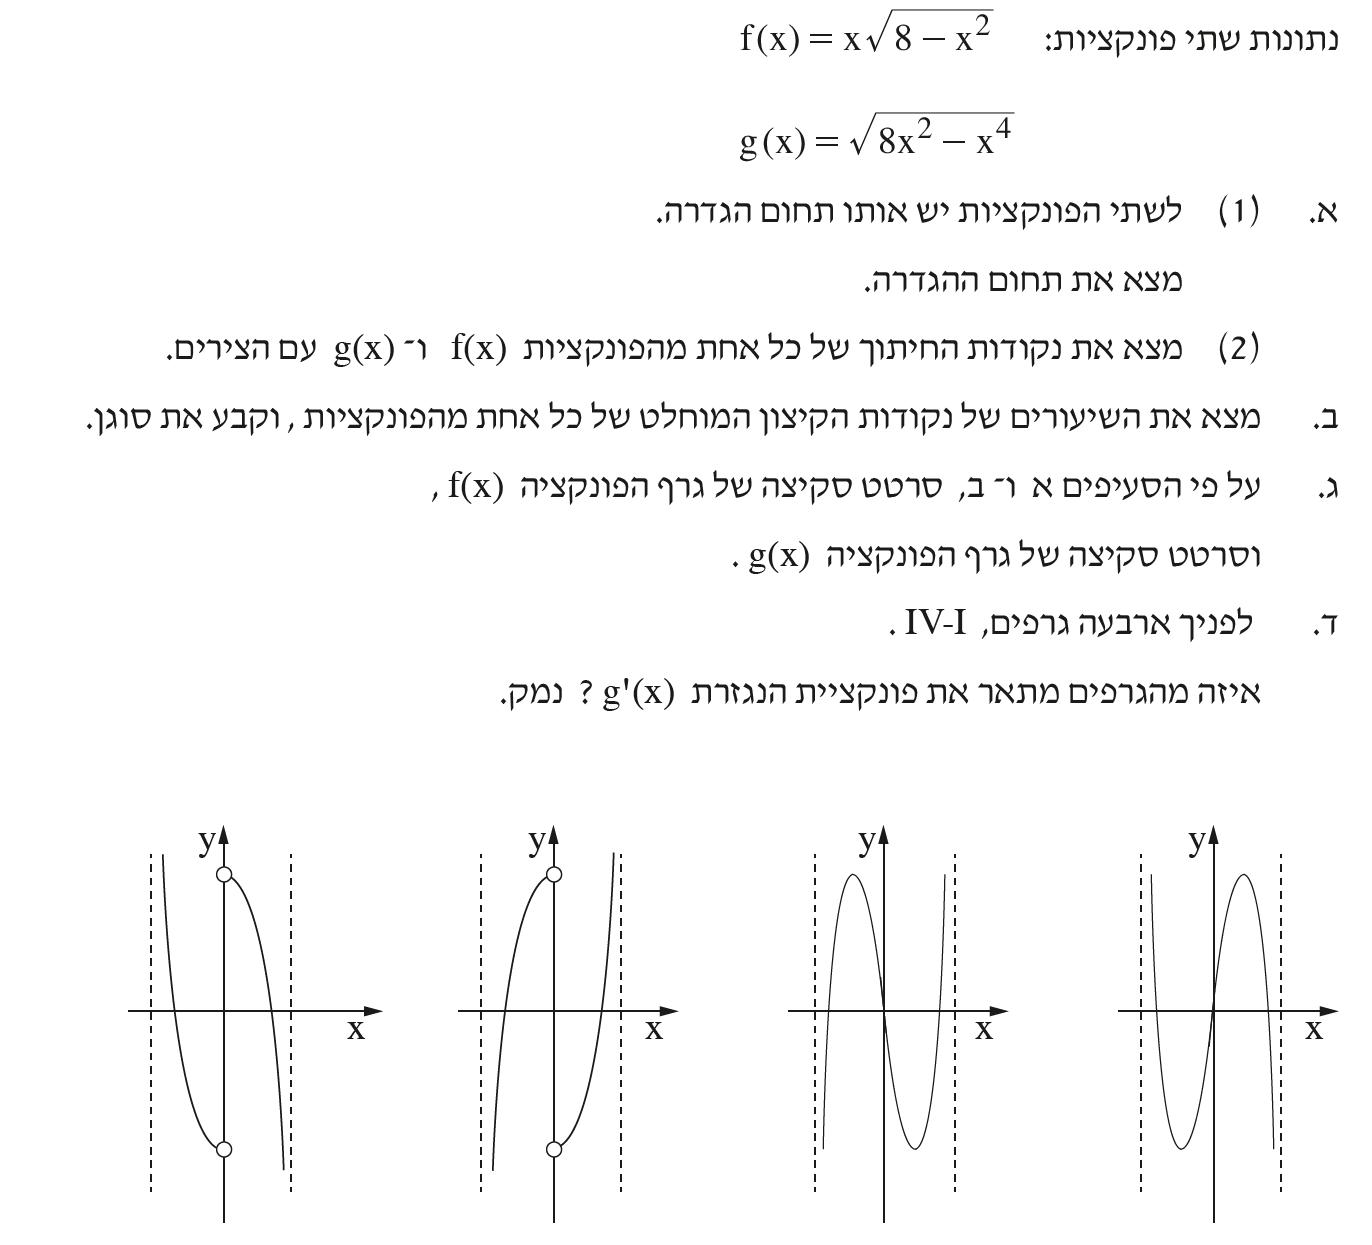
\includegraphics[width=\textwidth]{summer-2014b-6}
\end{center}

\vspace{-4ex}


\textbf{סעיף א}

$(1)$
הפונקיות מוגדרת כאשר ביטוי בשורש לא שלילי. עבור 
$f$
אם 
$8-x^2\ge 0$
ותחום ההגדרה הוא
$-\sqrt{8}\leq x \leq \sqrt{8}$.

עבור 
$g$
אם
$8^2-x^4\ge 0$
ותחום ההגדרה מורכב מ-%
$-\sqrt{8}\leq x \leq \sqrt{8}$
ו-%
$x=0$.
אבל 
$x=0$
נמצא בתוך התחום הראשון כך שהוא לא מוסיף ערכים לתחום ההגדרה, ותחומי ההגדרה של 
$f,g$
זהים.

$(2)$
עבור 
$f$:
אם 
$y=0$,
$x=0$
או
$\sqrt{8-x^2}=0$,
ונקודות החיתוך עם ציר ה-%
$x$
הן
$(0,0)$, $(\pm\sqrt{8},0)$.
אם 
$x=0$,
$y=0$
ונקודת החיתוך עם ציר ה-%
$y$
היא
$(0,0)$.

עבור
$g$:
אם 
$y=0$,
$\sqrt{8x^2-x^4}=\sqrt{x^2}\cdot\sqrt{8-x^2}=0$
עבור אותם ערכים
$0,\pm\sqrt{8}$.
ונקודות החיתוך הן אותן נקודות שקיבלנו עבור
$f$.

\np

\textbf{סעיף ב}

\vspace{-3ex}

\erh{14pt}
\begin{equationarray*}{rcl}
f'(x) &=& \sqrt{8-x^2} + x \cdot \frac{1}{2} \cdot \frac{1}{\sqrt{8-x^2}} \cdot (-2x)\\
&=&\frac{8-2x^2}{\sqrt{8-x^2}}\\
g'(x)&=&\frac{1}{2\sqrt{8x^2-x^4}}\cdot (16x-4x^3)\\
&=&\frac{8x-2x^3}{\sqrt{8x^2-x^4}}=\frac{x(8-2x^2)}{\sqrt{8x^2-x^4}}\,.
\end{equationarray*}

\vspace{-2ex}

פרט לנקודות הקצה
$\pm\sqrt{8}$
המכנה חיובי, אז הנגזרות יתאפסו כאשר המונה יתאפס. עבור 
$f$
הנקודות הן
$(-2,-4)$,$(2,4)$.
בנקודות הקצה,
$(\pm\sqrt{8},0)$,
ולכן
$(-2,-4)$
היא מינימום אבסולוטי )כי
$-4>0$(
ו-%
$(2,4)$
היא מקסימום אבסולוטי )כי
$4<0$(.
עבור 
$g$
הנקודות הן
$(0,0)$,$(-2,4)$,$(2,4)$.
בנקודות הקצה,
$(\pm\sqrt{8},0)$.
$(0,0)$, $(\pm\sqrt{8},0)$
הן מינימום אבסולוטי ו-%
$(-2,4)$,$(2,4)$
הן מקסימום אבסולוטי.


\textbf{סעיף ג}

נתבסס על תחומי ההגדרה ונקודות הקצה של הפונקציות כדי לציירן:

\begin{center}
\selectlanguage{english}
\begin{minipage}{.45\textwidth}
\begin{tikzpicture}[scale=.9]
\begin{axis}[
    ylabel = {$f(x)$},
    axis lines=center,
    xtick={-3,...,3},
    ytick={-4,...,4},
    xmin = -3.5,
    xmax = 3.5,
    ymin = -4.1,
    ymax = 4.1,
    xticklabel style={
    anchor=north east,
    },
    yticklabel style={
    anchor=south east,
    },
    every axis y label/.style={at={(axis cs:.7,3.5)}},
]
\addplot [
    domain=-2.828427:2.828427, 
    samples=60, 
]
{x*sqrt(8-x^2)};
\fill (axis cs:-2,-4) circle (1.5pt);
\fill (axis cs:2,4) circle (1.5pt);
\end{axis}
\end{tikzpicture}
\end{minipage}
\begin{minipage}{.45\textwidth}
\begin{tikzpicture}[scale=.9]
\begin{axis}[
    ylabel = {$g(x)$},
    axis lines=center,
    xtick={-3,...,3},
    ytick={-4,...,4},
    xmin = -3.5,
    xmax = 3.5,
    ymin = -4.1,
    ymax = 4.1,
    xticklabel style={
    anchor=north east,
    },
    yticklabel style={
    anchor=south east,
    },
    every axis y label/.style={at={(axis cs:.7,3.5)}},
]
\addplot [
    domain=-2.828427:2.828427, 
    samples=100, 
    style=thick,
]
{sqrt(8*x^2-x^4)};
\fill (axis cs:-2,4) circle (1.5pt);
\fill (axis cs:2,4) circle (1.5pt);
\end{axis}
\end{tikzpicture}
\end{minipage}
\end{center}


\textbf{סעיף ד}
\[
g'(x)=\frac{x(8-2x^2)}{\sqrt{8x^2-x^4}}
\]
לא מוגדר באפס, ולכן אפשר לפסול 
$III,IV$.
נחשב מספר ערכים:
\[
\erh{0pt}
\begin{array}{c|c|c|c|c}
x & -2 & -2 & 1 & 2\\\hline
g'(x) & 0 & -(6/7) & (6/7) & 0\\\hline
\end{array}
\]
הפונקציה יורדת כאשר מתקרבים לציר ה-%
$y$
משמאל וגם יורדת כאשר מתרחקים מהציר מימין. לכן הגרף
$I$
מתאר את הפונקציה.


%%%%%%%%%%%%%%%%%%%%%%%%%%%%%%%%%%%%%%%%%%%%%%%%%%%%%%%%%%%%%%%%%%%%%%


\section{קיץ תשע"ד מועד א}

\begin{center}
\selectlanguage{english}
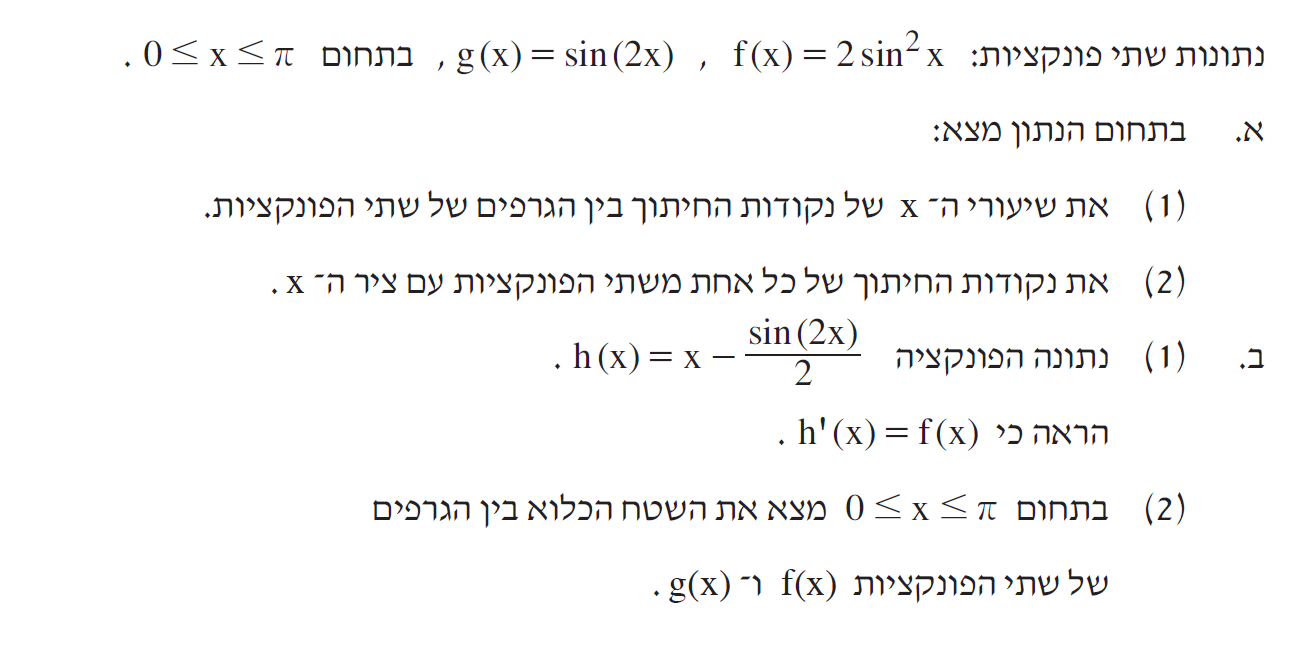
\includegraphics[width=\textwidth]{summer-2014a-6}
\end{center}

\vspace{-4ex}


\textbf{סעיף א}

$(1)$
ברור שערכי הפונקציות שווים ב-%
$x=0, x=\pi$
כי 
$\sin 0 = \sin \pi = 0$.
נשווה את המשוואות ונחפש פתרונות אחרים, כאשר נניח ש-%
$\sin x \neq 0$
(ולכן החילוק ב-%
$\sin x$
מותר(:
\erh{6pt}
\begin{equationarray*}{rcl}
2\sin^2 x &=& \sin 2x\\
&=& 2\sin x \cos x\\
\sin x &=& \cos x\\
x&=& \frac{\pi}{4}\,.
\end{equationarray*}

$(2)$
ראינו ששתי הפונקציות מקבלות ערך אפס ב-%
$0,\pi$.
נחפש ערכים אחרים בתוך התחום.

עבור 
$f$:$2\sin^2 x=0$
רק כאשר
$x=0,\pi$,
ולכן נקודות החיתוך עם ציר ה%
$x$
הן
$(0,0),(\pi,0)$.

עבור 
$g$:
$\sin 2x=0$
כאשר
$2x=0+k\pi$,
ולכן יש נקודות חיתוך גם ב-%
$(\frac{\pi}{2},0)$.

\textbf{סעיף ב}

$(1)$
\erh{12pt}
\begin{equationarray*}{rcl}
h(x)'=\left(x-\frac{\sin 2x}{2}\right)'&=& 1-\frac{2\cos 2x}{2}=1-\cos 2x\\
&=&1- (\cos^2 x - \sin^2 x)=(1- \cos^2 x) + \sin^2 x\\
&=&2\sin^2 x=f(x)\,.
\end{equationarray*}

\np

$(2)$
מהתרשים להלן אנו רואים שהשטח מורכב משני קטעים, מ-%
$0$
עד
$\frac{\pi}{4}$,
ומ-%
$\frac{\pi}{4}$
עד
$\pi$.
\begin{center}
\selectlanguage{english}
\begin{tikzpicture}[scale=.9]
\begin{axis}[
    trig format plots=rad,
    axis lines=center,
    xmin=-.1,
    xmax=3.141,
    xtick={0,.7854,1.571,2.356,3.141},
    xticklabels={$0$,$\frac{\pi}{4}$,$\frac{\pi}{2}$,$\frac{3\pi}{4}$,$\pi$},
    ymin = -2,
    ymax = 2,
    ytick={-2,...,2},
%    xticklabel style={anchor=north east,},
]
\addplot [
    domain=0:3.141, 
    samples=40, 
    name path=f,
]
{2*(sin(x))^2};
\addplot [
    domain=0:3.141, 
    samples=40, 
    name path=g,
]
{sin(2*x)};
\path[name intersections={of=f and g,by={a,b}}];
\draw[dashed,thick] (b) |- (axis cs:.7854,0);
\fill (axis cs:0,0) circle(2pt);
\fill (b) circle(2pt);
\fill (axis cs:3.141,0) circle(2pt);
\node at (axis cs:2.5,1.5) {$f(x)$};
\node at (axis cs:1.6,.7) {$g(x)$};
\end{axis}
\end{tikzpicture}
\end{center}
בסעיף זה יש מתנה: כדי לקבל האינטרגל של 
$f(x)$
נוכל להשתמש בפונקציה
$h(x)$
נתונה:
\[
h(x) = x-\frac{\sin 2x}{2} = \int h'(x) = \int f(x)\,.
\]
השטח הראשון הוא:
\erh{12pt}
\begin{equationarray*}{rcl}
\int_0^\frac{\pi}{4}(\sin 2x - f(x)) dx &=&\left.\frac{-\cos 2x}{2} - x +\frac{\sin 2x}{2}\right|_0^\frac{\pi}{4}\\
&=&\left(0-\frac{\pi}{4}+\frac{1}{2}\right)-\left(-\frac{1}{2}-0+0\right)=-\frac{\pi}{4}+1\,.
\end{equationarray*}

השטח השני הוא:
\erh{12pt}
\begin{equationarray*}{rcl}
\int_\frac{\pi}{4}^\pi (f(x)-\sin 2x) dx &=&x -\left.\frac{\sin 2x}{2}-\frac{-\cos 2x}{2}\right|_\frac{\pi}{4}^\pi\\
&=&\left(\pi-0+\frac{1}{2}\right)-\left(\frac{\pi}{4}-\frac{1}{2}+0\right)=\frac{3\pi}{4}+1\,.
\end{equationarray*}

השטח הכולל הוא:
\[
S=-\frac{\pi}{4}+1+\frac{3\pi}{4}+1=\frac{\pi}{2}+2\,.
\]


\section{חוקף תשע"ד}

\begin{center}
\selectlanguage{english}
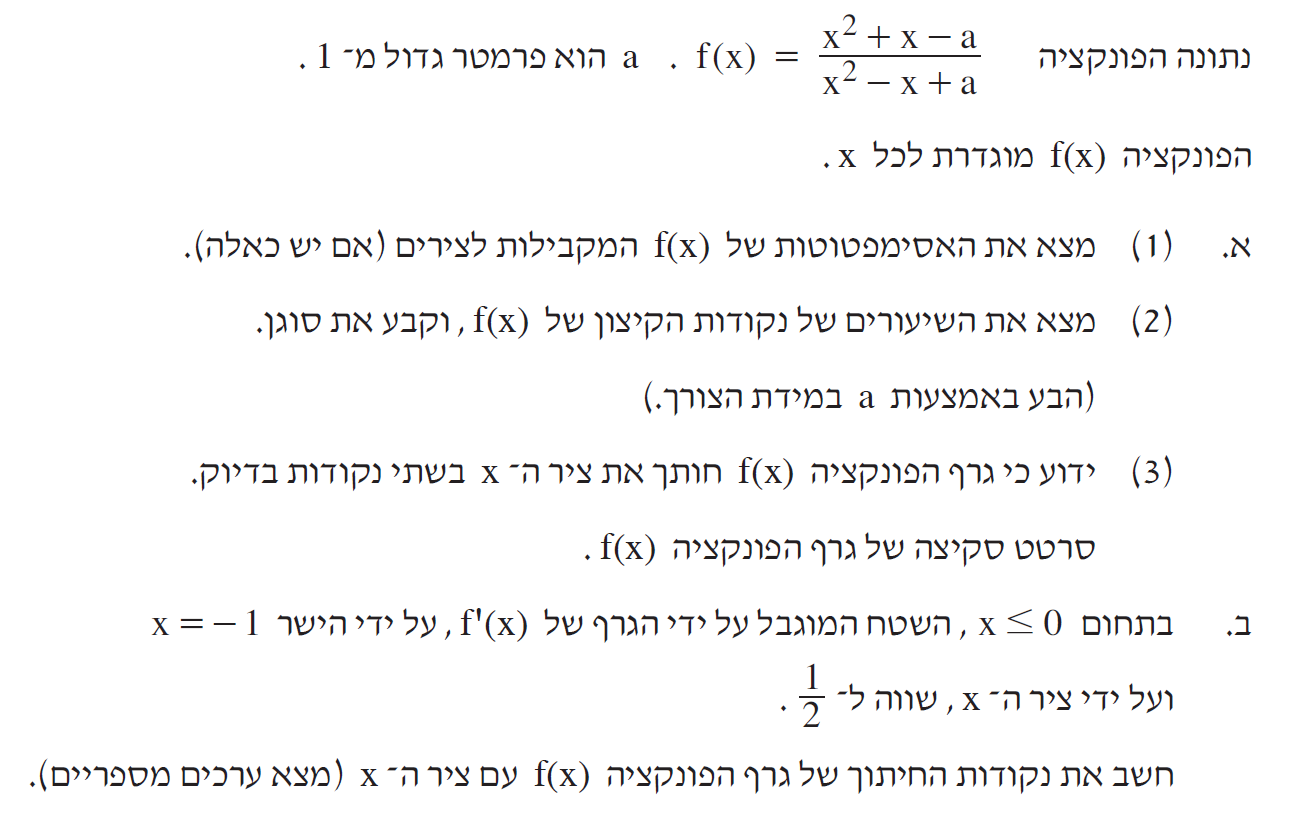
\includegraphics[width=\textwidth]{winter-2014-7}
\end{center}

\vspace{-4ex}

\textbf{בבחינה זו היו שלוש שאלות בפרק השני לכן מספר השאלה הוא 
$7$
ולא 
$6$.}

נתון שהפונקיה מוגדרת לכל 
$x$
אבל מתחשק לי לוודא שזה נכון. אם נשווה את המכנה לאפס נקבל משוואה ריבועית שפתרונה היא:
\[
\frac{1\pm\sqrt{1-4a}}{2}\,.
\]
נתון ש-%
$a>1$
אז אין פתרונות ממשיים למשוואה.

\textbf{סעיף א}

$(1)$
הפונקציה מוגדרת לכל 
$x$
אז אין 
\asms{}
אנכיות.

נחלק את הפונקציה בחזקה הגדולה ביותר ונקבל:
\[
\frac{1+\frac{1}{x}-\frac{a}{x^2}}{1-\frac{1}{x}+\frac{a}{x^2}}
\]
ששואף ל
$1$
כאשר 
$x\rightarrow \pm\infty$.
ה%
\asm{}
האופקית היא
$y=1$.


$(2)$
נחשב את הנגזרת הראשונה:
\[
f'(x) =\frac{(2x+1)(x^2-x+a)-(x^2+x-a)(2x-1)}{(x^2-x+a)^2}=\frac{-2x^2+4xa}{(x^2-x+a)^2}\,.
\]
מכנה חיובי ולכן הנגזרת תתאפס כאשר
$2x^2=4ax$.
נקודות הקיצון הן:
\[
(0,-1),\quad (2a,\frac{4a+1}{4a-1})\,.
\]

\np

המכנה של הנגזרת הראשונה חיובית ולכן מספיק לחשב את הנגזרת של המונה ולבדוק את הנימנה:
\[
(-2x^2+4ax)'=-4x+4a
\]
ב-%
$x=0$
$-4x+4a$
חיובי כי נתון ש-%
$a>1$,
ולכן נקודת הקיצון היא מינימום. ב-%
$x=2a$
$-8a+4a=-4a$
שלילי כי נתון ש-%
$a>1$,
ולכן נקודת הקיצון היא מקסימום.



$(3)$
קיים מינימום ב-%
$x=0$
ו%
\asm{}
אופקית ב-%
$y=1$.
לפי הנתון שיש שתי נוקודות חיתוך עם ציר ה-%
$x$,
הגרף עולה מנקודת המינימום ושואף לאינסוף ב-%
$y=1$.
נשאר רק להחליט אם נקודת המקסימום היא מעל ל%
\asm{}
או מתחתיה. אבל עם
$a>1$,
$\frac{4a+1}{4a-1}>1$
אז הנקודת המקסימום נמצאת מעל ל%
\asm{}.



\begin{center}
\selectlanguage{english}
\begin{tikzpicture}[scale=1]
\begin{axis}[
    xlabel = $x$,
    ylabel = {$f(x)$},
    axis lines=center,
    xtick={-5,...,5},
    ytick={-2,...,2},
    xmin = -5,
    xmax = 5,
    ymin = -2,
    ymax = 2,
%    xticklabel style={
%    anchor=north west,
%    },
%    yticklabel style={
%    anchor=north,
%    },
    every axis y label/.style={at={(ticklabel cs:0.8)},rotate=90,anchor=west,},
    every axis x label/.style={at={(ticklabel cs:0.8)},anchor=north,},
]
\addplot [
    domain=-5:5, 
    samples=50, 
]
{(x^2+x-2)/(x^2-x+2)};
\draw[dashed,thick] ({axis cs:-4,1}-|{rel axis cs:0,0}) -- ({axis cs:-4,1}-|{rel axis cs:8,0});
\fill (axis cs:0,-1) circle(1.5pt);
\fill (axis cs:1,0) circle(1.5pt);
\fill (axis cs:-2,0) circle(1.5pt);
\fill (axis cs:4,1.286) circle(1.5pt);
\end{axis}
\end{tikzpicture}
\end{center}


\textbf{סעיף ב}

האינטגרל של הנגזרת הראשונה הוא הפונקציה עצמה:
\[
\left|\int_{-1}^0 f'(x) dx\right| = \left.|\left.f(x)\right|_{-1}^0=f(0)-f(-1)\right|=\left|1-\frac{-a}{a+1}\right|=\left|\frac{-2}{a+2}\right|\,.
\]
נתון שהשטח שווה ל-%
$\frac{1}{2}$
ולכן 
$a=2$.
ערכי ה-%
$x$
של נקודות החיתוך הן הפתרונות של:
\[
x^2+x-2=0\,
\]
שהם
$x=1,x=-2$.
נקודות החיתוך הן
$(1,0), (-2,0)$.


%%%%%%%%%%%%%%%%%%%%%%%%%%%%%%%%%%%%%%%%%%%%%%%%%%%%%%%%%%%%%%%%%%%%%%
\section{המלצות}

\begin{itemize}
\item
אי-אפשר להכין טבלה של עליות וירידות עד שלא מחשבים את תחום ההגדרה וכל נקודות הקיצון של הפנוקציה, כי רק ביניהם אפשר לסמוך על זה שאין שינוי בכיוון הפונקציה.

\end{itemize}

\end{comment}


\selectlanguage{english}


\tikzsetfigurename{trig-functions}
% !TeX root = chapter-6-7-8.tex

\selectlanguage{hebrew}


\chapter{חקר פונקציות טריגונומטריות}

\np

\section{המלצות}


\selectlanguage{english}


\tikzsetfigurename{optimization}
% !TeX root = chapter-6-7-8.tex

\selectlanguage{hebrew}


\chapter{בעיות קיצון}

\np

\section{המלצות}


\selectlanguage{english}



\end{document}
